
%%%%%%%%%%%%%%%%%%%%%%%%%%%%%%%%%%%%%%%%%%%%%%%%%%%%%%%%%%%%%%%%%%%
%%%%%%%%%%%%%JIBLM Formatting Package%%%%%%%%%%%%%%%%%%%%%%%%%%%%%%
%%%%%%%%%%%%%Version 1.2: August, 2008%%%%%%%%%%%%%%%%%%%%%%%%%%%
%%%%%%%%%%%%%Author: Paul J. Kapitza, Berry College%%%%%%%%%%%%%%%%
%%%%%%%%%%%%%%%%%%%%%%%%%%%%%%%%%%%%%%%%%%%%%%%%%%%%%%%%%%%%%%%%%%%

\documentclass[oneside]{book}
%%%%%%%%%%%%%journal additions%%%%%%%%%%%%%%%%%%%%%%%%%%%%%%%%%%%%%
\usepackage{time}%make system time available
\usepackage{enumerate}%extended enumeration package
%%%%%%%%%%%%%Symbol libraries%%%%%%%%%%%%%%%%%%%%%%%%%%%%%%%%%%%%%
\usepackage{amssymb}
\usepackage{amsmath}
\usepackage{latexsym}
\usepackage{amsthm}%extended ams-theorem environment

\usepackage{lettrine}%Drop-caps for Masthead
\usepackage{mathptmx}%Times Roman type package for both math and text


\usepackage{endnotes}%Footnotes to the instructor.
   
   
   
   
%%%%%%%%%%%%%Header Customization%%%%%%%%%%%%%%%%%%%%%%%%%%%%%%%%%
\usepackage{fancyhdr}%Header customization
\pagestyle{fancy}
%%%%%%%%%%%%%Chapter headings%%%%%%%%%%%%%%%%%%%%%%%%%%%%%%%%%
\renewcommand{\chaptermark}[1] {\markboth{#1}{}}%

%%%%%%%%%%%%%Page Formatting%%%%%%%%%%%%%%%%%%%%%%%%%%%%%%%%%%
\setlength{\oddsidemargin}{63pt}%%%%%One-sided printing values for 10pt. text-Remove for two sided print
\setlength{\evensidemargin}{63pt}%%%%%One-sided printing values for 10pt. text-Remove for two sided print

\setlength{\parskip}{1mm}
\setlength{\textwidth}{5.0in}
\setlength{\textheight}{8.0in}

%%%%%%%%%%%%%%%%%%%%%%%%%%%%AUTHOR MASTHEAD%%%%%%%%%%%%%%%%%%%%%%%%%%%%%
\newcommand{\authormasthead}{
\begin{flushleft}
\hspace{8.0mm}
\rule{0.3\linewidth}{0.3mm}
\lettrine[lines=2]{D}{raft \rule[3pt]{10mm}{0.5pt} Draft \rule[3pt]{10mm}{0.5pt} Draft \rule[3pt]{10mm}{0.5pt} Draft}
\rule{0.3\linewidth}{0.3mm}
%\hspace{1mm} Issue~\textbf{#1}, Volume #2        Issue 1 (August, 2007)
\vspace{0.2in}
\end{flushleft}
}
%%%%%%%%%%%%%%%%%%%%%%%%%%%%AUTHOR MASTHEAD%%%%%%%%%%%%%%%%%%%%%%%%%%%%%

%%%%%%%%%%%%%%%%%%%%%%%%%%%%TIMESTAMP%%%%%%%%%%%%%%%%%%%%%%%%%%%%%
%%Uses the ``time" package to stamp the time-Editing Feature
\newcommand{\timestamp}{{Edited: \texttt{\now , \today}}}
%%%%%%%%%%%%%%%%%%%%%%%%%%%%TIMESTAMP%%%%%%%%%%%%%%%%%%%%%%%%%%%%%


\let\affiliation\date


%%%%%%%%%%%%%%%%%%%%%%%%%%%% TITLEPAGE%%%%%%%%%%%%%%%%%%%%%%%%%%%%%
%
\makeatletter
\def\maketitle{%
  \null
  \thispagestyle{empty}%
  \timestamp
  \authormasthead
  %\vfill
  \normalfont
  \vspace{2in}
\begin{center}\leavevmode
{\Huge \@title\par}%
\vspace{20mm}
{\Large \@author\par}%
\vspace{5mm}
{\Large \@date\par}% pass affiliation
{\Large \ }
\end{center}
  \vfill
  \null
  \cleardoublepage
 \let\newauthor\@author%transfer to footer line
 }%
\makeatother
%%%%%%%%%%%%%%%%%%%%%%%%%%%% END OF TITLEPAGE%%%%%%%%%%%%%%%%%%%%%%%%%%%%%

%Customized headers and footers- replace authorname with register
\lhead{ \leftmark} \chead{} \rhead{\thepage}
\lfoot{\newauthor} \cfoot{} \rfoot{\emph{DRAFT -- DRAFT -- DRAFT}}
\renewcommand{\headrulewidth}{0.4pt}
\renewcommand{\footrulewidth}{0.4pt}
%
%%%%%%%%%%%%%%%%%%%%%%%%%%%% Annotation Environment %%%%%%%%%%%%%%%%%%%%%%%%%%%%%
\usepackage{comment}
\newcommand{\InstructorVersion}{\includecomment{annotation}}
\newcommand{\StudentVersion}{\excludecomment{annotation}}
%%%%%%%%%%%%%%%%%%%%%%%%%%%% END OF Annotation Environment%%%%%%%%%%%%%%%%%%%%%%%%%%%%%



%%%%%%%%%%%%%%%%%%%%%%%%%%%% Begin--Sectioning Redefines%%%%%%%%%%%%%%%%%%%%%%%%%%%%%
%
\makeatletter
\renewcommand{\@makechapterhead}[1]{%
\vspace*{50\p@}%
  {\parindent \z@ \raggedright \normalfont
    \ifnum \c@secnumdepth >\m@ne
      \if@mainmatter
        \huge \@chapapp\space \thechapter                
        \par\nobreak
        \vskip 20\p@
      \fi
    \fi
    \interlinepenalty\@M
    \LARGE\bfseries  #1\par\nobreak                        
    \vskip 40\p@
  }}


\renewcommand{\@makeschapterhead}[1]{%
  \vspace*{50\p@}%
  {\parindent \z@ \raggedright
    \normalfont
    \interlinepenalty\@M
    \LARGE\bfseries  #1\par\nobreak                      
    \vskip 40\p@
  }}

\makeatother
%%%%%%%%%%%%%%%%%%%%%%%%%%%% End--Sectioning Redefines%%%%%%%%%%%%%%%%%%%%%%%%%%%%%




%%%%%%%%%%Theorem Environments%%%%%%%%%%%%%%%%%%%%%%%%
\newtheorem{theorem}{Theorem}
\newtheorem{acknowledgment}[theorem]{Acknowledgment}
\newtheorem{algorithm}[theorem]{Algorithm}
\newtheorem{axiom}[theorem]{Axiom}
\newtheorem{case}[theorem]{Case}
\newtheorem{claim}[theorem]{Claim}
\newtheorem{conclusion}[theorem]{Conclusion}
\newtheorem{condition}[theorem]{Condition}
\newtheorem{conjecture}[theorem]{Conjecture}
\newtheorem{corollary}[theorem]{Corollary}
\newtheorem{criterion}[theorem]{Criterion}
\newtheorem{definition}[theorem]{Definition}
\newtheorem{example}[theorem]{Example}
\newtheorem{exercise}[theorem]{Exercise}
\newtheorem{lemma}[theorem]{Lemma}
\newtheorem{notation}[theorem]{Notation}
\newtheorem{problem}[theorem]{Problem}
\newtheorem{proposition}[theorem]{Proposition}
\newtheorem{remark}[theorem]{Remark}
\newtheorem{solution}[theorem]{Solution}
\newtheorem{summary}[theorem]{Summary}
%%%%%%%%%%Theorem Environments%%%%%%%%%%%%%%%%%%%%%%%%
\usepackage[all]{xy}
\usepackage{color,graphicx}
%
%%%%%%%%%%%%%%%%%%%%% Annotation Environment Switch%%%%%%%%%%%%
%\StudentVersion
\InstructorVersion
%%%%%%%%%%%%%%%%%%%%% Annotation Environment Switch%%%%%%%%%%%%
%
\newcommand\Rn{$\mathbb{R}^n$}
\newcommand\Rm{$\mathbb{R}^m$}
\newcommand\R{$\mathbb{R}$}
\newcommand\bq{\begin{question}}
\newcommand\eq{\end{question}}
\newcommand\be{\begin{enumerate}}
\newcommand\ee{\end{enumerate}}
\newtheorem{question}[theorem]{Question}
\renewcommand{\labelenumi}{\alph{enumi})}
\newcount\colveccount
\newcommand*\colvec[1]{
        \global\colveccount#1
        \begin{bmatrix}
        \colvecnext
}
\def\colvecnext#1{
        #1
        \global\advance\colveccount-1
        \ifnum\colveccount>0
                \\
                \expandafter\colvecnext
        \else
                \end{bmatrix}
        \fi
}

\begin{document}
\large
\frontmatter
\title{Linear Algebra \\
Notes and Problems}
\author{Nicholas Long}
\affiliation{Stephen F. Austin State University}
\maketitle
\tableofcontents

\begin{annotation}
\chapter{To the Instructor}
I have written much of this introduction, as well as the instructor comments within the notes, highlighting some of the ideas that have worked well for me and the other professor who has used these notes. As always with materials for the classroom, your milage may vary. A guiding principle of active classrooms is to do what you think will work best. Many of the ideas stated here may be familiar to instructors experienced in running an inquiry oriented classroom, but I feel compelled to restate for clarity. 

This introduction will go over the course and student population that these notes were created for and used with, as well as describe how the course has been run. Additionally, I will highlight some of the difficulties and successes that have come from this approach to a junior level linear algebra course. Later, I have also included some of the variations that I have used in grading student work including rubrics. I have added comments on particular problems throughout the notes and these superscripts refer to endnotes in the last Chapter titled, “Notes to the Instructor.”

\section{Course Background}
These questions and notes were developed for use in a junior level linear algebra course at Stephen F. Austin State University (SFA). SFA is a medium-sized, comprehensive, regional state university in East Texas, with a mathematics and statistics department that graduates about 20 to 30 mathematics majors a year. Students are required to have an intro to proof course as a prerequisite and many have completed multivariable calculus. For many students, this is the first course that \emph{uses} proofs. In brief, students are familiar with the ideas around proofs, but they are not good at them. As such, the mechanics of conjecture, proofs, and counterexamples are incrementally built up over the course of these notes (more on this later). This linear algebra course serves both mathematics majors and minors and these notes have been used in four different sections over four years by two faculty members. Some of the students in these sections had an IBL-style intro to proofs course, but those that did not had likely never had a course outside of the traditional lecture model. The sections in which these notes were used varied from 12 to 25 students, with the greatest success around 15-18 students. The differential equations course at SFA is not tied to the linear algebra in sequence, so some students may have seen some mechanics and themes from linear algebra in the differential equations course, but they would not have developed the tools.

The content goal of this course is exposure to the ideas and methods of linear algebra, but some instructors at SFA rarely stray out of vectors in $\mathbb{R}^3$ and do not have students writing many of their own proofs. These notes take the approach that the vast uses and methods of linear algebra cannot be covered and understood by students in a single semester. As such, a deep understanding of the importance of fundamental concepts (efficiently solving systems of linear equations, vector spaces, linear transformations) is the focus of the notes, with digressions into some of the related topics (like LU-factorizations, solutions to differential equations, or directed graphs). These notes aim to go deep enough into the fundamentals that a student who is successful in this course can pick-up material that is not directly covered from any traditional linear algebra text fairly easily. These notes assume that students have some experience with manipulating vectors in $\mathbb{R}^2$ and $\mathbb{R}^3$ along with the basic linear geometry from a multivariable calculus course.

These notes are not constructed as a sequence of proofs to be worked through in sequence to discover linear algebra, but rather as a mix of calculation, examples/counterexamples, and proofs that are meant to guide students through the fundamentals of linear algebra with depth and an emphasis on connecting to previous ideas. For example, the material in Chapter 1 can be covered in two weeks in a traditional course (if you don't turn around from writing on the board). But in this approach takes a third of the course because of the habits of mind that we are attempting to cultivate and an emphasis on understanding connections between ideas. From a pedagogical standpoint, there is a focus on growth in students. Specifically, many students have a poor understanding of when they master material. As such, these notes are focused on helping students see the difference between being able to work through a few examples and being able to easily move mentally between general and specific cases. A typical development of a topic involves a definition, the student working through an example(s), generalizing by connecting to other topics, and finally applying that generalization to another example (possibly previewing some future area of work). The examples are almost always worked through by students and typically represent most of the possibilities for the topic. I have tried as much as possible to guide students through without expecting them to be clever. By this I mean that I am not trying to rely on students seeing the right \textit{'trick'} to do a problem but rather how the problem can naturally be solved with the available tools. By chapter 3, students have a greatly improved facility with working in the abstract and needing fewer examples (sometimes they see it without an example since they have a good idea of the possibilities).

While everything cannot be covered and is not even attempted in this set of notes, the in-class discussions offer the instructor the possibility to connect these ideas to broader mathematics on a daily basis. Further, the role of the instructor should include brief comments on filling in gaps in important ideas and explanations of notational conventions. In the notes, I have added some additional questions that can be discussed in class when there is additional time after student presentations and discussion. Sometimes these questions preview an idea that students may find useful in broader context but are not strictly necessary for the material in the notes.

\section{Classroom Mechanics}
In most semesters that these notes were used, a first day activity like Dana Ernst's \lq\lq{Setting the Stage}\rq\rq activity is used to engage the students in the pedagogy of active learning. In one semester, I handed out the first set of problems (Warmup Problems) and set students up in groups of three to start working. After about 20 minutes of work, I pointed out to students how much they are able to do on these problems without direct instruction and then set up how we will be working on similar questions for much of the course. The key aspects of the first day should be about students' ability to make progress without direct instruction and the importance of communication (both written and oral).

Every class meeting after the first day is similar and takes the flow of 1 )assignment of student presentations, 2) students at boards/remaining students working in pods, 3) oral student presentation/questions/discussions, 4) instructor questions/followup, 5) assignment for next meeting.
The two instructors that have used these notes used slightly different methods for assigning problems to be presented. Both instructors allowed students to sign up on the board for any proofs that are in the assigned set for that meeting and then assignments are made in reverse seniority. In other words, the student who signed up for a proof and had the fewest presentations gets the first attempt for that question. One instructor used a web based app to assign (non-proof) problems to random individuals or small groups, according to the relative difficulty or need to engage the whole class. The other instructor allowed students to sign up for any problem that was to be presented and then the instructor would assign problems by circling the name of the student selected to present to each question.
In these notes, students are expected to write up a complete proof for problems that use the word "prove" and enough work to demonstrate their line of thinking on any problem. The students generally adapt as they see presentations that are efficient and some that are deficient in either content or communication. Having the students writing what work they deem necessary on the board at the same time necessitates a lot of board space in the classroom, but allows for students who are not presenting to examine the ideas that the see are most pressing to them.

Once students come into class, they are not to write on their work except with felt tip markers (provided by the instructor). When students turn in their work each day, there is a record of the students' work in pen/pencil and the edits they make based on seeing presentations and discussing the questions. This mitigates the instructors need to write corrections on the homework and emphasizes the cyclical nature of working and editing in problem solving. Further, this normalizes the expectation that mastery does not happen after the first encounter, but rather by returning to these ideas. Both instructors allowed proofs to be resubmitted after the due date until they are done to a satisfactory level, but other problems are graded as a set according to a rubric presented below. This also gives a specific expectation for students who are not presenting, namely that they are discussing their difficulties, evaluating the work on the boards, and integrating any comments or changes into their own work. You will need to remind students that you expect work to be done outside of class and that they don't get credit if they didn't have sufficient effort documented before class.

Some fruitful wrinkles to employ involving students who are not presenting involve having small groups work through additional examples to be used in later discussions. The instructor will often split time between checking in with presenters and students who are not presenting to assess the efforts and help anyone get un-stuck (which can often take only about 30 seconds for individual interactions). Just as in the notes, the instructor will likely say a bit more at the start of the course than towards the middle and end.

Students will need reminders about the goals, expectations, and reasoning for the pedagogical approach. These should be done at the individual level and as a class, but need to be done regularly during the first half of the course. One of the most potent reminders is pointing out how much good work and understanding students are able to generate. Additionally, students find that they end up really thinking about math rather than trying to get an answer. Mike Starbird has a set of short videos on YouTube that give some main points of the book "Five Elements of Effective Thinking" by Burger and Starbird. I have had good success with having students watch these and give a short written reflection on what they think of the ideas presented in the video. I use a couple of other reflective exercises when I anticipate that student will become frustrated with their increased involvement in the running of the course. 

I have a couple of rules that have helped me in deciding when to talk and what to talk about when it comes to the in-class discussions and the instructor questions/followup. The first thing to remember is to not say anything that a student can say. By this I mean that as an instructor, you should speak when what needs to be said can only come from the instructor. Allowing students the space and time to understand and state a question or problem with material being presented is central to active, inquiry based classrooms. It can be very hard to understand when you need to intervene but setting the tone that student commentary is needed and expected early in the course is essential. One way in which I think you should be free to comment and can often stir conversation is to discuss notation and mathematical conventions with students. This is something that I don't think students can comment easily on and they would benefit greatly from having guidance on. For example, you might complement on how a student made good choices in the notation or wording in the presentation of a question, then talk about how the choices of the presenter guide the reader in how they thought about and approached the question. You should take the time to name as much as possible after students and give student as much credit as possible for their propositions. I have found it useful to have some intermediate questions in my head at the start of class so that if the conversation stalls, you can posit a question that everyone is on equal footing for (unprepared students should be able to contribute as much as a prepared student). With the additional time left in class after student presentations, I will either get students started on the next set of problems (so that I can head off any stumbling blocks early in the problem set) or breifly introduce the next concept through the gap in knowledge that would be helpful to have filled. For instance, when starting the idea of span of a set of vectors, I like to have a discussion on how many vectors can be generated from linear combinations of just two vectors. 


\section{Student Expectations and Grading}
One of the greatest challenges for me in an inquiry based classroom is getting students to quickly understand and adapt to the expectations, which are very different than the other college level mathematics courses. I try, with all assignments and material given to them, to stress that the students' thoughts are the most valuable contribution they can give to the course. We discuss the thinking behind a problem, not just the answer because outside the classroom they will be expected to make progress on problems for which answers are unknown. There is also the expectation that students will be respectful and supportive of other students and their ideas. If students feel like they are in front of judges instead of coaches, you will not have the free exchange of ideas that is necessary for students to thrive in this setting. 

Students are expected to work, both individually and as a group, on effective thinking and communication of their thoughts. It needs to be explicitly said that this will be an area for growth (through effort) throughout the semester. Students are not expected to be perfect at the start of the course, but rather through the work and discussions required in-class they should see many examples (both good and bad) which they can use to improve. Since both the content and meta-goals of this course require regular work to improve, students are expected to turn in their work every class. Each assignment should not be overwhelming and allow students some additional time (especially later in the course) to reflect and rework old proofs. 

From a mathematical content perspective, linear algebra offers a set of topics that is very coherent and should offer students the opportunity to see how material fits together. Very often students have a "fake it until you make it" philosophy that can get them through lower level mathematics courses that are lecture driven. If students do not make the transition to sense-making rather than answer-getting, later mathematics course can be very painful experiences. The first step is make sure that students know the material should make sense and is not a set of topics that is "happening to them." I believe that linear algebra is a great place for students see how a subject should make sense as an evolution from solving useful problems and generalizing to an abstract setting. More than in any other mathematical field, linear algebra works the way we hope and expect that it should. 

I have found the following rubrics useful for grading and explaining that a one out of two on a homework assignment does not mean that you got half the problems correct. I include the following passage on my syllabus and will print out and pass out slips with this rubric when I think students need a reminder about what feedback I am trying to give (above the written feedback on assignments.)

Homework sets will be graded on a scale of 0 to 3. (I reserve the right to assign 4 points to an exceptionally well written homework set!) You should not think of the grade of an individual assignment as representing a percentage of questions that you got the right answer for, but rather as delivering a message about the problem solving process:
\newline
\begin{tabular}{|l|p{11cm}|}
\hline
3 & Student work is complete, including justification or explanation of the processes in solving problems. The work may not be completely correct but the work demonstrates a good line of reasoning. \\
\hline
2 & Student work is mostly complete and all problems have been attempted including some justification or explanation of the process of solving the problem.\\
\hline
1 & Student work is incomplete, lacking explanations, or not an adequate attempt at solving problems. \\
\hline
0 & Student work is missing or does not represent an adequate attempt at solving problems. \\
\hline
\end{tabular}

Remember that your Presentations/Homework grade will include points for presenting and working on problems at the board. In general, you should be getting more problems properly solved and justified than not in order to pass this class.
Proofs will be graded on a scale of 0 to 2. (I reserve the right to assign 3 points to an exceptionally well written or elegant proof!) You should \textbf{not} think of the grade as representing a percentage but, rather, as delivering a message:
\newline
\begin{tabular}{|l|p{11cm}|}
\hline
2 & great work; no real complaints on content or on writing.\\
\hline
1 & argument basically correct but missing some details\{\}less clearly argued than I would like. A correct but especially poorly written proof might merit a 1 as well.\\
\hline
0 & Serious errors or gaps in the mathematics or justification. This includes the problem being completely wrong or not done at all.\\
\hline
\end{tabular}

Remember that you can resubmit proofs.
\end{annotation}

\chapter{To the Student}

In this course, you will learn about linear algebra by solving a carefully designed sequence of problems.  It is important that you understand \textbf{every} problem and proof. As hard as it is to imagine, you will occasionally want to have more questions to work on in order to fully understand the ideas in this class. Feel free to ask me about additional problems to consider when you are stuck. The notes and problems will refer back to previous parts, so I suggest you keep a binder with the notes and your work together and bring all of these materials to class and any office hours. I also suggest having several colored pens or pencils to help you draw and label your work so it will be easily understood. Your written work needs to be legible and large enough so that someone else can easily read and understand what you are doing.

Unlike mathematics courses you have had in the past, solving a problem in this course will \textbf{always} have two components:
\begin{itemize}
\item Find a solution
\item Explain how you know that your solution is correct.
\end{itemize}
This will help prepare you to use mathematics in the future, when there will \underline{not} be someone to tell you if your solution is correct (or not). That is also why it will be primarily up to you (the students) to assess the correctness of work done and presented in class. This means that using the proper language (both written and spoken) and specificity are keys to effective communication. This class will teach you about the specificity and precision of mathematical language, so it is important that you practice and work on this. In order for you to understand the ideas in this class you will need to evaluate other people's ideas as well as your own for correctness. The work in this class is \emph{not about getting an answer} but rather \textbf{making sense} of the process and ideas involved in the problems. For this reason, justification in your work and ideas is very important. Why you did or tried something is just as important as what you did or what result you got. In fact, clearly articulating your thought process will make you a more efficient thinker.

\textbf{You are not alone in this course.} The role of the instructor is to guide the discussion and make sure you have the resources to be successful. While this new learning environment can be a bit unsettling for students at first, you will get comfortable as you do more problems and get feedback from other students and the instructor. \underline{I am also here to help you outside of class time} and expect you to find a way to get the help you need, whether face to face or over email. You will find that once you have thought about a problem for a little while, it will only take a little push to get unstuck.

Some Notation:
\begin{itemize}
\item $\mathbb{N}=\{0,1,2,3,...\}$ is the set of natural numbers
\item $\mathbb{Z}=\{...-3,-2,-1,0,1,2,3,...\}$ is the set of integers
\item $\mathbb{R}$ is the set of real numbers
\item $\mathbb{R}^n$ is the set of vectors with $n$ components from $\mathbb{R}$. $\mathbb{R}^n$ can also be viewed as the set of points in $n$-space. For instance, $\mathbb{R}^2$ would be the cartesian plane and $\mathbb{R}^3$ would correspond to three dimensional space
\item $\mathbb{C}=\{a+b i | a,b \in \mathbb{R}\}$ is the set of complex numbers
\item $A$, $B$, $C$, ... denote matrices
\item $\vec{u}$, $\vec{v}$, $\vec{w}$, ... denote vectors (which starting in Chapter 2 will not necessarily be in $\mathbb{R}^n$)
\item $\vec{0}_V$ is the zero vector in vector space $V$
\item $\emptyset$ is the null set or set that contains no elements
\item $M_{m \times n}$ is the set of matrices with $m$ rows and $n$ columns
\item DNMS is an acronym for \textit{Does Not Make Sense}
\item DNE is an acronym for \textit{Does Not Exist}
\end{itemize}
Definitions will be bolded for some terms and others will have their own heading and number. Many definitions and comments will be numbered so that everyone will be able to refer to them in work.

You will need to make some plots in this class and it will be advantageous to use a computer algebra system in some problems. For this reason, I suggest that, if you have not already, you should make an account on CoCalc at https://cocalc.com/ (fromerly the Sage MathCloud at https://cloud.sagemath.com). Additionally, CoCalc will allow you to easily write your work in LaTeX, a wonderful typesetting program. A homework bonus will be given to students who write their work in LaTeX.


\mainmatter

\chapter{Efficiently Solving Systems of Linear Equations and Matrix Operations}



\section{Warmup Problems}
\begin{annotation}
\endnote{I use this set of problems to emphasize that students already have experience with linear algebra problems and that we will be looking to classify all possibilities in related problems.}
\end{annotation}
\begin{question} Solve:
$$ 3x_1-2x_2=6 $$
$$-x_1+x_2=1 $$
\end{question}

\begin{question} Draw a graph of the solution set of the equation: $3x_1-2x_2=6$ (Hint: If a solution has $x_1=a$, what is $x_2$ or viceversa?)
\end{question}

\begin{question} Draw a graph of the solution set of the equation: $-x_1+x_2=1$
\end{question}

\begin{question}\label{q2} Graph the solution sets from Questions 2 and 3 together. How does your answer to Question 1 compare to your graph?
\end{question}

\begin{question} Solve:
$$ 2x_1-2x_2=6 $$
$$-x_1+x_2=1 $$
\end{question}

\begin{question} Solve:
$$ 2x_1-2x_2=-2 $$
$$-x_1+x_2=1 $$
\end{question}

\begin{question} Wait... what just happened? Explain the results of the previous two problems. What do the graphs of the corresponding solution sets look like in relation to the graphs of the equations?
\end{question}

\begin{question} What are the possible intersections of two lines? Clearly state your conjecture.
\end{question}

Throughout this course we will be doing many of the same things you did in the previous questions, but we will do them in a more general setting that will allow us to solve \textbf{many} new and old problems.

\newpage
\section{Solving Linear Systems}
Our first chapter will cover the ideas of efficiently solving a system of linear equations and matrix operations.

A system of $m$ linear equations in $n$ variables can be written:

\begin{equation*}
\setlength{\arraycolsep}{2pt}
\begin{array}{rcrcrcrcr}
  a_{11} x_1  &+& a_{12} x_2 &+& ... &+&  a_{1n}x_n &=& b_1 \\
  a_{21} x_1  &+& a_{22} x_2 &+& ... &+&  a_{2n}x_n &=& b_2 \\
  \vdots  & & \vdots & &  & &  \vdots &&  \\
  a_{m1} x_1  &+& a_{m2} x_2 &+& ... &+&  a_{mn}x_n &=& b_m
\end{array}
\end{equation*}
The term $a_{ij}$ is the \textbf{coefficient} of the $j$-th variable (denoted $x_j$) in the $i$-th equation. A \textbf{solution} is a choice of variable values that satisfies all equations in the system. A solution is \emph{not} a particular variable value but must include a choice for \underline{all} variables in the system. The \textbf{solution set} for a system of equations is the set of all possible solutions. We will have many ways to describe solutions to a system this semester but they all specify the values of $x_1$, $x_2$, ..., and $x_n$, typically as an ordered $n$-tuple ($x_1$, $x_2$, ..., $x_n$).

\bq Is $(1,2,3)$ a solution to the following system?
\begin{equation*}
\setlength{\arraycolsep}{2pt}
\begin{array}{rcrcrcrcr}
  1 x_1  &+& 2 x_2 &+& 3 x_3 &=& 14 \\ % -1  3
  2 x_1  &-& 3 x_2 &+& 2 x_3 &=& 0 \\
   x_1   & &       &+& 7 x_3 &=& 0
\end{array}
\end{equation*}
\eq

The previous problem shows how easy it is to check if a set of variable values is a solution. However, \emph{finding} a solution or the set of all solutions is harder but very important to many problems. Generally speaking, the process of finding the solution set for a system of equations is to trade the system of equations you have for an \textbf{equivalent} system (a system with the same solution set).

\bq For each pair of equations given, state whether $E_1$ is equivalent to $E_2$.
\be
\item $E_1: x^2-1=0$ \hfill $E_2: x-1=0$
\item $E_1: x^2-2x+1=0$ \hfill $E_2: x-1=0$
\item $E_1: e^x=1$ \hfill $E_2: x^3+x^2+x=0$
\ee \eq


Hopefully it will be easier to explicitly write the solution set of the new equivalent system. An \textbf{elementary operation} on a system of equations is an operation of the form:
\begin{enumerate}
\item multiplying an equation by a non-zero scalar
\item switching two equations
\item adding a multiple of one equation to another equation
\end{enumerate}

\begin{question}
For this question, we will consider the following system of linear equations:
$$a_1 x_1+a_2x_2+a_3x_3=a_4$$
$$b_1 x_1+b_2x_2+b_3x_3=b_4$$
\begin{enumerate}
\item Multiply the second equation in our system by negative three and state the \textbf{new} system of equations.
\item Write a few sentences about why the new system of equations given in the previous part is equivalent to the original system.
\item Write a few sentences about why switching the order in which equations are presented in a system does not change the set of solutions.
\item Write out the equation obtained by multiplying the second equation in the original system by a non-zero scalar (which we will call $k$) and adding to the first equation.
\item Replace the second equation in the original system with your answer to the previous part, which we will call System 2. Prove that System 2 is equivalent to the original system. In other words, you need to show that $(c_1,c_2,c_3)$ is a solution of the equations $S_1$:
    $$a_1 x_1+a_2x_2+a_3x_3=a_4$$
    $$b_1 x_1+b_2x_2+b_3x_3=b_4$$
    \emph{if and only if} $(c_1,c_2,c_3)$ is a solution to System 2.
\end{enumerate}

\end{question}


%\begin{question} Given a set of equations in three variables show that elementary operations give an equivalent system of equations. In other words, you need to show that $(c_1,c_2,c_3)$ is a solution of the equations $S_1$:
%$$a_1 x_1+a_2x_2+a_3x_3=a_4$$
%$$b_1 x_1+b_2x_2+b_3x_3=b_4$$
%\emph{if and only if} $(c_1,c_2,c_3)$ is a solution to the equations obtained after performing one of the operations above. Hint: For each type of elementary operation, write out the new system given by performing the given operation on $S_1$ and then show that the new system is equivalent. It may help to try part $c)$ first.
%\end{question}

\begin{remark}
For those of you new to the term \lq\lq \textbf{if and only if}\rq\rq (sometimes abbreviated \textbf{iff}), if and only if denotes a biconditional statement. A statement of the form \lq\lq P iff Q\rq\rq implies \lq\lq if P, then Q\rq\rq and \lq\lq if Q, then P\rq\rq. If you are asked to prove a biconditional statement you need to prove \textbf{both} conditional statements. The good news is that if you have a biconditional statement as a theorem, then you can use either (or both) of the conditional statements in your work.
\end{remark}
\begin{question}\label{q1} Solve the following systems just using elementary operations. Remember to show your work.
\begin{enumerate}
\item $$ 2y+z=4$$
$$x-3y+2z=5$$
$$2x+y =-2$$
\item $$3x-2y-z=0$$
$$2x+y+z=10$$
$$x+4y+3z=20$$
\item $$3x-2y-z=0$$
$$2x+y+z=10$$
$$x+4y+3z=10$$
\end{enumerate}
\end{question}

A system of equations is \textbf{consistent} if there exists at least one solution to the system. In other words, a consistent system of equations has a nonempty solution set. A system that is not consistent is said to be \textbf{inconsistent}.

In Question \ref{q1}, note that you didn't change anything but the coefficients in the system of equations as you traded one system for another. Some of the coefficients probably became zero but you didn't really eliminate any variables or consider a totally different problem. We will use matrices to efficiently store, and manipulate the coefficients in a system of linear equations, since they are all that matter for now. Matrices will have \emph{many} uses in this and other courses, and we will use capital letters like $A$ and $B$ to denote matrices. Matrices will be rectangular arrays with the same number of entries in each row and the same number of entries in each column. The size of a matrix is given (in order) as the number of rows by the number of columns, so a $3$ by $2$ matrix has $3$ rows and $2$ columns.

In order to specify what \textbf{entry} we are referring to in a matrix, we need an ordered pair of indices telling us the number of the row and number of the column to look in respectively. For instance, if $B=\begin{bmatrix} 1&5&0\\\heartsuit&\bigstar &\blacklozenge \\ \pounds&\circledR&\maltese \end{bmatrix}$, then the $(3,2)$ entry of $B$ is in the third row and 2nd column. You could also write this as $(B)_{3,2}= \circledR$. The \textbf{$i$-th row} of a matrix $A$ will be denoted $row_i(A)$ and the \textbf{$j$-th column} will be denoted $column_j(A)$.

In order to distinguish \textbf{vectors} (as being more than just $n$ by $1$ matrices), we will use the arrow notation and lower case symbols like $\vec{u}$ and $\vec{v}$ to denote vectors. Unless otherwise stated, we will use column vectors. For instance, if $\vec{v} =\colvec{4}{v_1}{v_2}{\vdots}{v_m}$, then the second \textbf{component} of $\vec{v}$ is the scalar $v_2$. The size of a vector in $\mathbb{R}^n$ is the number of components the vector has. In Chapter 2, we will deal with a \emph{much} more general notion of vectors that will \emph{not} have components like vectors in $\mathbb{R}^n$.

The \textbf{coefficient matrix} of a linear system of $m$ equations in $n$ variables is a $m$ by $n$ matrix whose $(i,j)$ entry is the coefficient of the $j$-th variable, $x_j$, in the $i$-th equation of the system. The \textbf{augmented matrix} of a linear system of $m$ equations in $n$ variables is a $m$ by $(n+1)$ matrix whose first $n$ columns are the coefficient matrix of the system and the last column is the constant terms from the right side of each equation.

The system
\begin{equation*}
\setlength{\arraycolsep}{2pt}
\begin{array}{rcrcrcrcr}
  a_{11} x_1  &+& a_{12} x_2 &+& ... &+&  a_{1n}x_n &=& b_1 \\ % -1  3
  a_{21} x_1  &+& a_{22} x_2 &+& ... &+&  a_{2n}x_n &=& b_2 \\
  \vdots  & & \vdots & &  & &  \vdots && \vdots \\
  a_{m1} x_1  &+& a_{m2} x_2 &+& ... &+&  a_{mn}x_n &=& b_m
\end{array}
\end{equation*}
has a coefficient matrix
$$A=\begin{bmatrix} a_{11} & a_{12} & ... &  a_{1n} \\
  a_{21}& a_{22}& ... &  a_{2n} \\
  \vdots  & \vdots &   &  \vdots   \\
  a_{m1}& a_{m2} & ... &  a_{mn}  \end{bmatrix}$$
and an augmented matrix of
$$[A|b]=\begin{bmatrix} a_{11} & a_{12} & ... &  a_{1n} &|&b_1\\
  a_{21}& a_{22}& ... &  a_{2n} &|&b_2\\
  \vdots  & \vdots &   &  \vdots &|& \vdots  \\
  a_{m1}& a_{m2} & ... &  a_{mn} &|&b_m \end{bmatrix}$$

For some properties of the system of equations, we need only look at the coefficient matrix but others will need the augmented matrix. It is important to know the difference and be able to state which corresponding matrix you are using in your work.

\begin{question} What is the coefficient matrix for the previous systems? Give the coefficient matrix for Question $i$ as $A_i$. (Hint: You should have 10 answers to this question from Questions 1, 2, 3, 5, 6, 9, 10, 11, and three from Question 13.)
\end{question}

\begin{question} What is the augmented matrix for the previous systems? Give the augmented matrix for Question $i$ as $A_i$. (Hint: You should have 10 answers to this question.)
\end{question}

The elementary operations on equations outlined above will correspond to elementary row operations on matrices as well. Specifically,
an \textbf{elementary row operation} on a matrix is an operation of the form:
\begin{itemize}
\item multiplying a row by a non-zero scalar
\item switching two rows
\item adding a multiple of one row to another row
\end{itemize}
We now have operations to trade our system of equations for an equivalent system, but we have not stated a way to make sure that the solution set will be easy to explicitly state from our new equivalent system. The following matrix forms will be useful for determining solution sets and various other properties of the corresponding system of equations.

\begin{definition}
A rectangular matrix is in \textbf{row echelon form} if it has the following three properties:
\begin{enumerate}
\item All nonzero rows are above any rows of all zeros.
\item Each \textbf{leading entry} (being the first non-zero entry) of a row is in a column to the right of the leading entry of the row above it.
\item All entries in a column below a leading entry are zeros.

If a matrix in row echelon form satisfies the following additional properties, then we say the matrix is in \textbf{reduced row echelon form}:

\item The leading entry in each nonzero row is 1.
\item Each leading 1 is the only nonzero entry in its column.
\end{enumerate}
\end{definition}

The leading entry in a nonzero row of the row echelon form is called a \textbf{pivot}. The column in which a pivot occurs is called a \textbf{pivot column} and the corresponding variable is a \textbf{basic variable} or \textbf{pivot variable}. A variable corresponding to a column in which the coefficient matrix does \underline{not} have a pivot are called \textbf{free variables}. While the echelon form is needed to find where pivots will occur, we will sometimes refer to pivot positions of a matrix even when the matrix is not in echelon form.

\begin{theorem} The reduced row echelon form of a rectangular matrix is unique.
\end{theorem}
It is important to note that the row echelon form of a matrix is \underline{not} unique.
\begin{question} Give an example of a matrix $M$ that has the following properties. If such a matrix cannot exist, explain why.
\begin{enumerate}
\item $M$ satisfies properties a and b of row echelon form but does not satisfy property c.
\item $M$ satisfies properties a and c of row echelon form but does not satisfy property b.
\item $M$ satisfies properties b and c of row echelon form but does not satisfy property a.
\item $M$ satisfies properties a, b, and c of row echelon form but does not satisfy property d of reduced row echelon form.
\item $M$ satisfies properties a, b, c, and d of reduced row echelon form but does not satisfy property e of reduced row echelon form.
\end{enumerate}
\end{question}

\begin{question}\label{q5} List out all possible row echelon forms of 3 by 4 matrices using the symbols $\blacksquare$ for a pivot, $*$ for a non-pivot entry (possibly $0$), and $0$ (when an entry \underline{must} be $0$). For each of these, list out which variables are pivot variables and which are free variables. Hint: There are 15 possible.
\end{question}

\begin{question} List out all possible reduced row echelon forms of 3 by 4 matrices using the symbols $\blacksquare$ for a pivot, $*$ for a non-pivot entry (possibly $0$), and $0$ (when an entry \underline{must} be $0$). What value must the $\blacksquare$ entries be? For each of these, list out which variables are pivot variables and which are free variables.
\end{question}

\begin{question}\label{q3} Solve each of the following systems by converting to an augmented matrix and using elementary row operations to reduce the augmented matrix to reduced row echelon form. With each reduced row echelon form, put a box around all pivot entries. Use the system of equations corresponding to the reduced row echelon form to write out the solution set for each system.
\begin{enumerate}
\item  $$ 3x_1-2x_2=6$$
$$ 2x_1-2x_2=-2 $$
$$-x_1+x_2=1 $$
\item  $$ 3x_1-2x_2=6$$
$$ 2x_1-2x_2=6 $$
$$-x_1+x_2=1 $$
\item  $$4x-y+3z=5$$
$$3x-y+2z=7$$
\item  $$7x-11y-2z=3$$
$$8x-2y+3z=1$$
\item  $$3r-5s+t=2$$
$$-6r+10s-2t=3$$
\end{enumerate}
\end{question}
\begin{question}
Given an augmented matrix $[A|b]$ and its row reduced echelon form $[A'|b']$, write a procedure (set of steps) to give the solution set to the corresponding systems of equations. Make sure you are clear in writing out your steps.

Are there any ways in which your procedure will fail to work? Are there any systems whose augmented matrices will not have a reduced row echelon form?
\end{question}



Two of the most important questions we will consider this semester are:

1) Is the system consistent?

2) If a solution exists, is the solution unique?

\begin{question} Look back at your results so far and try to figure out what properties of the system (or corresponding matrices) will help us answer question 1 and which properties of the system will help us answer question 2. Write a conjecture about each question. \end{question}

The space below is for you to write a statement of the theorem that the class decides is the best for determining consistency and uniqueness.
\begin{theorem}
Classwide statement of consistency theorem:
\vspace{2.5in}

\end{theorem}

\begin{theorem}
Classwide statement of uniqueness theorem:
\vspace{2.5in}

\end{theorem}

The following two proofs are difficult and one of the reasons we will be resubmitting proofs.
\begin{annotation}
\endnote{This ends up being a great place to talk about being careful about what exactly is being said. In student work, you will often see phrases like "matrix is unique" or "matrix is consistent".  This is a great time to talk to students about kinds of objects and the properties of an object type. For instance, a matrix cannot be consistent but a system of equations can be. A matrix can be unique but more often than not the student means that the associated system of equations has a unique solution. One of the great struggles in these junior level courses is getting students into the habit of editing their work with precision.

It is not uncommon for the class to have to work and rephrase even their best attempts at the consistency and uniqueness theorems. I will allow them to change these theorems later in the course if they see why they need to.

The next two questions can be left out. The proof are rarely completed by any but the most persistent students and require a facility with proof techniques that many students have seen but not internalized yet. Hand-waving versions of the proofs can be presented fairly easily. Your mileage may vary.}
\end{annotation}
\bq Prove the classwide statement of the consistency theorem.
\eq
\bq Prove the classwide statement of the uniqueness theorem.
\eq
\bq Using the statement of the classwide uniqueness and consistency theorems, treat each of your answers to Question \ref{q5} as a \underline{coefficient} matrix of a linear system of equations and state:
\begin{enumerate}
\item whether each corresponding system of equations will be consistent, inconsistent, or you can't tell.
\item whether each corresponding system of equations will have a unique solution, multiple solutions, no solutions, or you can't tell.
\end{enumerate}
\eq
\bq Using the statement of the classwide uniqueness and consistency theorems, treat each of your answers to Question \ref{q5} as an \underline{augmented} matrix of a linear system of equations and state:
\begin{enumerate}
\item whether each corresponding system of equations will be consistent, inconsistent, or you can't tell.
\item whether each corresponding system of equations will have a unique solution, multiple solutions, no solutions, or you can't tell.
\end{enumerate}
\eq

\subsection{Geometric Interpretation of a Solution Set}

Recall from Questions 2 through 8, that the solution set of a linear equation in two variables was a line in $\mathbb{R}^2$ (the plane) and that the solution set of a system of two equations in two variables was possibly a point, a line, or empty. Similarly, the solution set for a linear equation in three variables will be a plane in 3-space ($\mathbb{R}^3$).

\begin{question}\be
\item List out all the possible ways two planes can intersect in a three dimensional space.
\item List out all the possible ways three planes can intersect in a three dimensional space.
\item List out all the possible ways four planes can intersect in a three dimensional space.
\item List out all the possible ways five planes can intersect in a three dimensional space.
\begin{annotation}
\endnote{This question usually precipitates a discussion of what intersection means. Some students will say that you are considering the intersection of all the objects in a collection and others may say that you can consider anywhere that at least two of the objects have in common. I like to use this as motivation for why we are using IBL and talking about things "everyone already knows." I like to mention how having seen a topic is different than having made sense of definition and examples.}
\end{annotation}
\ee\end{question}

We don't usually draw what a solution set of a linear equation in four variables looks like because drawing in four dimensions is difficult. The graph would be called a hyperplane in $4$-space. For the same reasons, we certainly don't draw $m$ hyperplanes in $n$-space but the solution sets work very similar to the pictures we can draw in 3-space (also known as $\mathbb{R}^3$).

\bq Why does the graph of a linear equation in $n$ variables need to be a flat $n-1$ dimensional hyperplane?
\eq
Recall that the following commands will plot the plane given by $3x-2y-z=0$ in Sage:

\verb" var('x,y'); "

\verb"plot3d(3*x-2*y,(x,-10,10),(y,-10,10),color='red') "

Plotting the equations, $3x-2y-z=0$, $2x+y+z=10$, and $x+4y+3z=20$ in red, yellow, and green respectively gives:

\begin{center}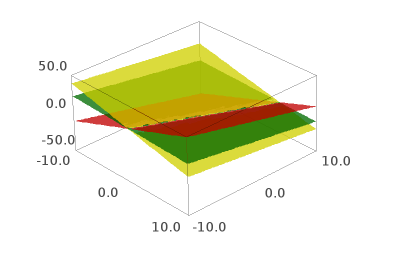
\includegraphics[scale=1.5]{3planeplot.png}\end{center}

\begin{question} Does your answer to Question \ref{q1} part b make sense with this plot? Explain.
\end{question}

\bq For each of the systems in Question \ref{q3}, use Sage to draw a plot of each of the equations in the system and write a sentence for each system about why the plot and your answer to Question \ref{q3} make sense.
\eq

If you remember parametric equations of lines and planes in space from multivariable calculus, then we will return to those ideas in Section \ref{s1}.

\section{Vector and Matrix Equations}
Recall that two vectors in $\mathbb{R}^n$ are equal if and only if all of their components are equal.

\bq\label{q41} Prove that the system of equations given by
\begin{equation*}
\setlength{\arraycolsep}{2pt}
\begin{array}{rcrcrcrcr}
  a_{11} x_1  &+& a_{12} x_2 &+& ... &+&  a_{1n}x_n &=& b_1 \\ % -1  3
  a_{21} x_1  &+& a_{22} x_2 &+& ... &+&  a_{2n}x_n &=& b_2 \\
  \vdots  & & \vdots & &  & &  \vdots && \vdots \\
  a_{m1} x_1  &+& a_{m2} x_2 &+& ... &+&  a_{mn}x_n &=& b_m
\end{array}
\end{equation*}

has the same set of solutions as the vector equation

$$x_1 \colvec{4}{a_{11}}{a_{21}}{\vdots}{a_{m1}}+x_2 \colvec{4}{a_{12}}{a_{22}}{\vdots}{a_{m2}}+ \cdots x_n \colvec{4}{a_{1n}}{a_{2n}}{\vdots}{a_{mn}}=\colvec{4}{b_1}{b_2}{\vdots}{b_m}$$
In other words, prove that $(c_1,c_2,...,c_n)$ is a solution to the vector equation iff $(c_1,c_2,...,c_n)$ is a solution to the system of linear equations. Make sure you clearly connect the ideas in your proof and do not make an argument that these equations look similar.
\eq

\bq Solve the following vector equation directly:
$$x_1 \colvec{2}{1}{1}+x_2 \colvec{2}{-1}{1} = \colvec{2}{3}{-4}$$
\eq

\bq Give an example of a vector $\colvec{3}{a}{b}{c}$ such that the equation $$x_1\colvec{3}{1}{1}{0}+x_2 \colvec{3}{0}{0}{1}=\colvec{3}{a}{b}{c}$$ has no solution, or explain why no such vector exists.
\eq

\bq Give an example of a vector $\colvec{3}{a}{b}{c}$ such that the equation $$x_1\colvec{3}{1}{1}{0}+x_2 \colvec{3}{0}{0}{1}=\colvec{3}{a}{b}{c}$$ has exactly 1 solution, or explain why no such vector exists.
\eq

\bq Give an example of a vector $\colvec{3}{a}{b}{c}$ such that the equation $$x_1\colvec{3}{1}{1}{0}+x_2 \colvec{3}{0}{0}{1}+x_3 \colvec{3}{1}{1}{1}=\colvec{3}{a}{b}{c}$$ has exactly 1 solution, or explain why no such vector exists.
\eq

\bq Give an example of a vector $\colvec{3}{a}{b}{c}$ such that the equation $$x_1\colvec{3}{1}{1}{0}+x_2 \colvec{3}{0}{0}{1}+x_3 \colvec{3}{1}{1}{1}=\colvec{3}{a}{b}{c}$$ has no solutions, or explain why no such vector exists.
\eq

\bq Give an example of a vector $\colvec{3}{a}{b}{c}$ such that the equation $$x_1\colvec{3}{1}{1}{0}+x_2 \colvec{3}{0}{0}{1}+x_3 \colvec{3}{a}{b}{c}=\colvec{3}{7}{0}{-2}$$ has exactly 1 solution, or explain why no such vector exists.
\eq

\begin{definition} A \textbf{linear combination} of a set $S$ is a vector of the form $$\sum_{i=1}^n c_i \vec{v_i} = c_1 \vec{v_1} + c_2 \vec{v_2}+...+c_k \vec{v_k}$$ where $\vec{v}_i \in S$. Note that $$\sum_{i=1}^n c_i \vec{v_i}$$ will not usually be in $S$ even though $\vec{v}_i \in S$. \end{definition}

\bq Can you write $\vec{b}=\colvec{2}{2}{4}$ as a linear combination of $\vec{v_1}=\colvec{2}{1}{1}$ and $\vec{v_2}=\colvec{2}{-1}{1}$? Justify your answer.
\eq

\bq Repeat the previous problem for $\vec{b}=\colvec{2}{0}{0}$ and $\vec{b}=\colvec{2}{3}{-1}$.
\eq

\bq Can you write $\vec{b}=\colvec{3}{2}{0}{4}$ as a linear combination of $\vec{v_1}=\colvec{3}{1}{1}{1}$ and $\vec{v_2}=\colvec{3}{-1}{1}{1}$? Justify your answer.
\eq

\begin{definition}
We define a \textbf{matrix-vector product} as follows:

If $A$ is a $m$ by $n$ matrix, $$A=\begin{bmatrix} a_{11} & a_{12} & ... &  a_{1n} \\
  a_{21}& a_{22}& ... &  a_{2n} \\
  \vdots  & \vdots &   &  \vdots   \\
  a_{m1}& a_{m2} & ... &  a_{mn}  \end{bmatrix}$$ and $\vec{x}=\colvec{4}{x_1}{x_2}{\vdots}{x_n} \in \mathbb{R}^n$, then the \textbf{matrix-vector product} is given by $$A\vec{x} = x_1 \colvec{4}{a_{11}}{a_{21}}{\vdots}{a_{m1}}+x_2 \colvec{4}{a_{12}}{a_{22}}{\vdots}{a_{m2}}+ \cdots x_n \colvec{4}{a_{1n}}{a_{2n}}{\vdots}{a_{mn}}$$

%Note that the result of $A\vec{x}$ is an element of $\mathbb{R}^m$.
\end{definition}
\bq If $A$ is a $m$ by $n$ matrix, then $A\vec{x} \in \mathbb{R}^\diamondsuit$ for what value of $\diamondsuit$?
\eq

It should not surprise you that you can multiply a scalar multiple of a vector by a matrix by factoring out the scalar. In mathematical notation, $A (k \vec{v}) = k (A\vec{v})$. Additionally, you can apply the scalar multiplication to the matrix. In other words, $A (k \vec{v}) = k (A\vec{v}) = (kA)\vec{v}$. These kind of manipulations will be discussed more when we work with matrix operations later, but you may find these facts useful in your work right now.

\bq
\be
\item Write out the $k$-th component of the resulting vector of the product $$ \begin{bmatrix} a_{11} & a_{12} & ... &  a_{1n} \\
  a_{21}& a_{22}& ... &  a_{2n} \\
  \vdots  & \vdots &   &  \vdots   \\
  a_{m1}& a_{m2} & ... &  a_{mn}  \end{bmatrix} \colvec{4}{x_1}{x_2}{\vdots}{x_n}$$
\item How can you express the result of the matrix-vector product in terms of $\vec{x}$ and the rows of $A$?
\item How can you express the result of the matrix-vector product in terms of $\vec{x}$ and the column of $A$?
\ee
\eq

Based on the above definition of the matrix vector product, if $$A=\begin{bmatrix} a_{11} & a_{12} & ... &  a_{1n} \\
  a_{21}& a_{22}& ... &  a_{2n} \\
  \vdots  & \vdots &   &  \vdots   \\
  a_{m1}& a_{m2} & ... &  a_{mn}  \end{bmatrix}$$ and $\vec{b}= \colvec{4}{b_1}{b_2}{\vdots}{b_m}$, then by Question \ref{q41}, $A\vec{x} = \vec{b}$ has the same solution set as the system
\begin{equation*}
\setlength{\arraycolsep}{2pt}
\begin{array}{rcrcrcrcr}
  a_{11} x_1  &+& a_{12} x_2 &+& ... &+&  a_{1n}x_n &=& b_1 \\ % -1  3
  a_{21} x_1  &+& a_{22} x_2 &+& ... &+&  a_{2n}x_n &=& b_2 \\
  \vdots  & & \vdots & &  & &  \vdots && \vdots \\
  a_{m1} x_1  &+& a_{m2} x_2 &+& ... &+&  a_{mn}x_n &=& b_m
\end{array}
\end{equation*}


\bq Write each of the following as a matrix equation, a vector equation, and system of equations. You need to write out the exact corresponding vector equation, matrix equation, and system of equations, \underline{not} some equivalent form.
\begin{enumerate}
\item $\begin{bmatrix} 1 & 2& 3\\4&5&6\\7&8&9 \end{bmatrix} \colvec{3}{x_1}{x_2}{x_3} =\colvec{3}{a}{b}{c}$
\item $a_1 \colvec{3}{1}{2}{5}+\colvec{3}{3}{0}{-1}+a_2 \colvec{3}{-1}{0}{2} =\colvec{3}{4}{5}{0}$
\item $$ 2x_1+3x_2=7 $$ $$-x_1+x_2+4x_3=0 $$ $$ 5x_1-6x_2-x_3=2 $$
\end{enumerate}
\eq


\section{Solution Sets of Linear Systems}\label{s1}
In this section, we will talk about efficient and clear ways to express the set of solutions to a linear system of equations.
\bq Prove that if a system of linear equations has two distinct solutions, then the system has infinitely many solutions.
\eq

\bq\label{q12} For each of the systems in Question \ref{q3}, use the reduced row echelon form to solve for each pivot (basic) variable in terms of the free variables and constant terms. By substituting in your new expressions for the pivot variables into the vector $\colvec{4}{x_1}{x_2}{\vdots}{x_n}$, you will get a vector solely in terms of the free variables. You can now write the solution set as a linear combination of vectors with each free variable as a coefficient. For instance, if a system had free variables $x_2$ and $x_5$, then the parametric form would look like $\vec{u}+x_2 \vec{v}+ x_5 \vec{w}$. This is called the \textbf{parametric form} of the solution set for the system, and is really a linear combination of the vectors $\vec{u}$, $\vec{v}$, and $\vec{w}$ in the example.
\begin{annotation}
\endnote{It may be helpful to work through the first example of the previous question as a class to aid the students into seeing the form given in the problem.}
\end{annotation}
\eq

\bq\label{q4} Solve each of the following systems and present your solution set in parametric form.
\begin{enumerate}
\item  $$ 3x_1-2x_2=0$$
$$ 2x_1-2x_2=0 $$
$$-x_1+x_2=0 $$
\item  $$ 3x_1-2x_2=0$$
$$ 2x_1-2x_2=0 $$
$$-x_1+x_2=0 $$
\item  $$4x-y+3z=0$$
$$3x-y+2z=0$$
\item  $$7x-11y-2z=0$$
$$8x-2y+3z=0$$
\item  $$3r-5s+t=0$$
$$-6r+10s-2t=0$$
\end{enumerate}
\eq
\begin{definition}
A system of linear equations is \textbf{homogeneous} if the matrix form of the system, $A\vec{x} =\vec{b}$ has $\vec{b} =\vec{0}=\colvec{3}{0}{\vdots}{0}$. If $\vec{b} \neq \vec{0}$, then the corresponding system is \textbf{nonhomogeneous}.
\end{definition}
\bq\label{q7} Using your answers to Questions \ref{q12} and \ref{q4} as a guide, state and prove a theorem that discusses how the solution set to a homogeneous system is related to the solution set of the non-homogenous system.
\eq

\bq \emph{State and prove} a theorem that describes under what conditions of the matrix $A$ the system $A\vec{x}=\vec{b}$ will have a solution for every $\vec{b}$. Essentially, you need to fill in the blank of the following statement: If \underline{\hspace{2.5in}}, then $A\vec{x}=\vec{b}$ will have a solution for every $\vec{b} \in \mathbb{R}^m$.
\eq

\begin{definition} The \textbf{column space of a matrix} $A$, denoted $Col(A)$ is the set of vectors that can be written as a linear combination of the columns of $A$. If $A$ is $m$ by $n$, then $Col(A)=\{\vec{b} \in \mathbb{R}^m | A\vec{x} =\vec{b} \mbox{ for some } \vec{x} \in \mathbb{R}^n \}$.
\end{definition}

\begin{theorem} The pivot columns of a matrix $A$ generate $Col(A)$. This means that if $\vec{v} \in Col(A)$, then $\vec{v}$ can be written as a linear combination using only the pivot columns of $A$.
\end{theorem}
Note that this theorem uses the pivot columns of $A$ and \underline{\textbf{not}} the pivot columns of the \emph{echelon form} of $A$. Even though you need the echelon from to figure out which columns have pivots, you should use the appropriate columns of $A$ in your linear combination.


\begin{definition} The \textbf{null space of a matrix}, denoted $Null(A)$, is the set of vectors that when multiplied by the matrix give the zero vector. In other words, $Null(A)$ is the solution set of the homogeneous equation $A\vec{x}=\vec{0}$.
\end{definition}

\bq Let $A=\begin{bmatrix} 1&2&3 \\4&5&6 \end{bmatrix}$. Describe the sets $Col(A)$ and $Null(A)$ using a parametric form.
\eq

\bq Let $A=\begin{bmatrix} 1&2\\ 3&4\\5&6 \end{bmatrix}$. Describe the sets $Col(A)$ and $Null(A)$ using a parametric form.
\eq

\bq Let $$A=\begin{bmatrix} -3&6&-1&1&-7&0 \\1&-2&2&3&-1&0 \\2&-4&5&8&-8&0 \end{bmatrix}  \thicksim \begin{bmatrix} 1&-2&0&-1&0&0\\0&0&1&2&0&0 \\ 0&0&0&0&1&0 \end{bmatrix}$$
What is the reduced row echelon form of $\begin{bmatrix} -3&-1&1 \\1&2&3 \\2&5&8\end{bmatrix}$? You should use the information given above and \textbf{not} a lot of calculations.
\eq

\bq Let $$A=\begin{bmatrix} -3&6&-1&1&-7 \\1&-2&2&3&-1 \\2&-4&5&8&-8 \end{bmatrix} \thicksim \begin{bmatrix} 1&-2&0&-1&0\\0&0&1&2&0 \\ 0&0&0&0&1 \end{bmatrix}$$
Describe $Col(A)$ and $Null(A)$ using a parametric form using as \underline{few} vectors as possible.
\eq

\bq Under what conditions on a $m$ by $n$ matrix,$A$, will $Col(A)$ be all of $\mathbb{R}^m$?
\eq

Remember that $Col(A)$ and $Null(A)$ are usually very different sets, in fact, they aren't always in the same parent set. If $A$ is a $m$ by $n$ matrix, then $Col(A)$ is in $\mathbb{R}^{\spadesuit}$ and $Null(A)$ is in $\mathbb{R}^{\clubsuit}$, for what values of $\clubsuit$ and $\spadesuit$?

\bq Find an example of a $2$ by $2$ matrix where $Col(A)$ is the same set as $Null(A)$.
\eq

\bq Given a matrix $A$ with echelon form $\begin{bmatrix} \blacksquare&*&*&*\\0&0&\blacksquare&* \\ 0&0&0&0 \end{bmatrix}$:
\be
\item What is the minimum number of vectors that will be needed to give the parametric form of $Col(A)$?
\item What is the minimum number of vectors that will be needed to give the parametric form of $Null(A)$?
\item $Col(A)$ is a subset of $\mathbb{R}^\spadesuit$ for what value of $\spadesuit$?
\item $Null(A)$ is a subset of $\mathbb{R}^\spadesuit$ for what value of $\spadesuit$?
\ee
\eq

\bq Given a matrix $A$ with echelon form $\begin{bmatrix} 0&\blacksquare&*&*&*\\0&0&0&\blacksquare&* \\ 0&0&0&0&0 \end{bmatrix}$:
\be
\item What is the minimum number of vectors that will be needed to give the parametric form of $Col(A)$?
\item What is the minimum number of vectors that will be needed to give the parametric form of $Null(A)$?
\item $Col(A)$ is a subset of $\mathbb{R}^\spadesuit$ for what value of $\spadesuit$?
\item $Null(A)$ is a subset of $\mathbb{R}^\spadesuit$ for what value of $\spadesuit$?
\ee
\eq
\bq\label{q10} Write a sentence to explain your answer to each part of the following question. Given a matrix $A$, how many vectors will be needed to give the parametric form of
\begin{itemize}
\item $Col(A)$
\item $Null(A)$
\end{itemize}
\eq
\bq Can every vector in $\mathbb{R}^3$ be written as a linear combination of the columns of $A = \begin{bmatrix} 1&5&-2&0 \\ -3&1&9&-5 \\ 4&8&-1&7 \end{bmatrix}$? Justify your answer.
\eq

\section{Applications}
Solving linear systems of equations can be used to balance equations of chemical reactions. For instance, if propane ($C_3H_8$) and oxygen ($O_2$) react to give off carbon dioxide ($CO_2$) and water ($H_2O$), you can write something like $C_3H_8 +O_2 \rightarrow CO_2+H_2O$ but this is not balanced because there are three carbon atoms going into this reaction and only one coming out. Instead we look at $x_1 (C_3H_8) +x_2 (O_2) \rightarrow x_3(CO_2)+x_4(H_2O)$, where $x_i$ stands for the number of molecules of each reactant needed to balance the chemical equation. We can then solve a system of equations where each equation comes from balancing a different element involved in the reaction.
\begin{annotation}
\endnote{These applications are nice for showing students how solving linear systems comes up in other areas of study, but are not essential for this course.}
\end{annotation}

\bq Give the system of equations described by the burning of propane above. Solve the system and check that this balances the chemical equation.
\eq

\bq Balance the following equations:
\begin{enumerate}
\item $B_2S_3 +H_2O \rightarrow H_3BO_3+H_2S$
\item $KMnO_4+MnSO_4+H_2O \rightarrow MnO_2+K_2SO_4+H_2SO_4$
\end{enumerate}
\eq

\bq Should the systems used to balance a chemical equation have a unique solution? Why or why not? Consider how many equations you will have and how many variables.
\eq

\bq In studying the urban-rural migration patterns of Springfield, you notice that in any given year 70\% of the population in urban areas stays in urban areas, 20\% moves to suburban areas, and 10\% moves to rural areas. For the population in a suburban area, the respective percentages moving to urban, suburban, and rural areas are 5\%, 80\%, and 15\%. For the population in a rural area, the respective percentages are 11\%, 14\%, and 75\%.
\be
\item If $u_t$, $s_t$, and $r_t$ are the percentages of the population in an urban, suburban, and rural areas in year $t$, set up a system of linear equations for $u_{t+1}$, $s_{t+1}$, and $r_{t+1}$ in terms of $u_t$, $s_t$, and $r_t$.
\item Write your answer to part $a)$ as a matrix equation where $\vec{x}_{t}=\colvec{3}{u_t}{s_t}{r_t}$ and $\vec{x}_{t+1}=\colvec{3}{u_{t+1}}{s_{t+1}}{r_{t+1}}$.
\item Use Sage to compute $\vec{x_1}, \vec{x_2},...,\vec{x_{10}}$, when $\vec{x_0}=\colvec{3}{.4}{.2}{.4}$.
\ee
\eq

\bq \label{q8} Networks (traffic, electrical, etc.) can be studied by setting up a system of linear equations corresponding to the different junctions. Specifically, at each junction, the amount of stuff coming in (flow in) must be the same as the amount of stuff going out (flow out). If $x1, ... , x9$ are the amount of stuff flowing between junctions, set up a system of equations corresponding to the network given below.

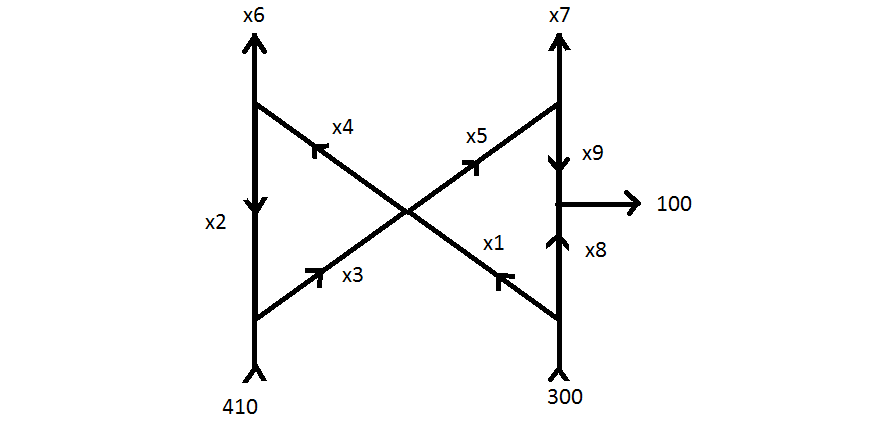
\includegraphics[scale=.5]{network.png}
\eq

\bq Is there only one way that the flow of stuff can satisfy the information given by the network graph above? Why or why not?
\eq

\bq Bonus: Solve the system of equation that is your answer to Question \ref{q8}. Describe how the parts of your solution set correspond to the network.
\eq

\section{Matrix operations}\label{mo}
\bq Finish the following sentences.
\be
\item Vectors are equal if ...
\item Matrices are equal if ...
\item A scalar is ...
\ee
\eq

Just as you can add two vectors in $\mathbb{R}^n$ componentwise, you can add two matrices entry-wise. For this reason, it only makes sense to add two matrices if they are the same size. You can also define scalar multiplication of a matrix entry-wise.
\begin{annotation}
\endnote{This section mixes some computation, understanding of notation, and basic proofs. This should serve as a foundation for success and real understanding (not faking it) in preparation for the abstract work done in Chapter 2.}
\end{annotation}

\bq Let $A=\begin{bmatrix} 3&-1&0 \\2&0&-7 \\ 4&2&6 \end{bmatrix}$, $B=\begin{bmatrix} 6&-2&0 \\3&0&-21 \\ 4&2&6 \end{bmatrix}$, \break and $C=\begin{bmatrix} 1&0&0 \\0&1&0\\1&1&1 \end{bmatrix}$.
\begin{enumerate}
\item Is $B$ a scalar multiple of $A$? Why or why not?
\item $2A-3C=$
\item $-(A+C)+2B=$
\item $(84A+16B-12C)_{2,1}=$
\end{enumerate}
\eq
\bq Symbolically, $(A+B)_{i,j}=\underline{\hspace{1.0in}}$ and $(k A)_{i,j}=\underline{\hspace{1.0in}}$
\eq
\begin{definition}
Let $A$ be a $m$ by $n$ matrix. The transpose of $A$, denoted $A^T$, is a $n$ by $m$ matrix such that $(A^T)_{ij}= (A)_{ji}$.
\end{definition}
There are a couple of ways to think about the transpose. First, you can think about flipping the matrix across the main diagonal (the elements of the form $A_{i,i}$). You can also view the transpose of a matrix as switching the rows and columns (but preserving the order). In other words, the $i$-th row of $A^T$ is the $i$-th column of $A$.

\bq Let $A=\begin{bmatrix} 3&-1 \\2&0 \\ 4&2 \end{bmatrix}$ and $B=\begin{bmatrix} 6&-2&0 \\3&0&-21 \end{bmatrix}$
\begin{enumerate}
\item $A^T=$
\item $B^T=$
\item $A^T+B=$
\item $B^T+A=$
\end{enumerate}
\eq

\bq Let $A=\begin{bmatrix} 3&-1&0 \\2&0&-7 \\ 4&2&6 \end{bmatrix}$, $B=\begin{bmatrix} 6&-2&0 \\3&0&-21 \\ 4&2&6 \end{bmatrix}$, \break and $C=\begin{bmatrix} 1&0&0 \\0&1&0\\1&1&1 \end{bmatrix}$.
\begin{enumerate}
\item $A+B^T=$
\item $((C-B)^T+A)^T=$
\end{enumerate}
\eq

\bq Prove that $(A+B)^T=A^T+B^T$ where $A$ and $B$ are $m$ by $n$ matrices.
\eq

\bq What dimensions should $A$ have in order to be able to add $A$ to $A^T$?
\eq

\bq Prove that $(A^T)^T=A$.
\eq

A matrix $A$ is \textbf{symmetric} if $A^T=A$.
\bq Prove that the sum of two symmetric $m$ by $n$ matrices is symmetric.
\eq

\bq Prove that $kA$ is symmetric if $A$ is symmetric. \eq


\subsection{Special Types of Matrices}
A \textbf{square} matrix is a matrix that has the same number of rows and columns. A $m$ by $n$ matrix $A$ is said to be \textbf{upper triangular} if $(A)_{ij}=0$ whenever $i>j$. Similarly, a matrix $A$ is \textbf{lower triangular} if $(A)_{ij}=0$ whenever $i<j$. We usually consider square matrices when we talk about upper or lower triangular, but it may be helpful to consider non-square cases.

\bq Give an example of a matrix that is upper triangular but is not in echelon form. If one does not exist, explain why.
\eq

\bq Give an example of a matrix that is in echelon form but is not upper triangular. If one does not exist, explain why.
\eq

\bq Can a matrix be upper \underline{and} lower triangular? Either give an example or explain why there cannot exist one.
\eq

\textbf{Diagonal} matrices are matrices whose only nonzero entries are on the diagonal. Specifically, a matrix $A$ is diagonal if $(A)_{ij}=0$ whenever $i \neq j$.

\bq Give an example of a matrix that is diagonal but not in echelon form.
\eq
The $n$ by $n$ identity matrix, denoted $Id_n$, is the unique matrix such that $Id_n \vec{x}= \vec{x}$ for every $\vec{x} \in \mathbb{R}^n$. In fact the entries of $Id_n$ are easily computed in terms of the Dirac delta function. Specifically $(Id_n)_{i,j}=\delta_{i,j}$, where $$\delta_{i,j}=\left\{ \begin{array}{cc} 0 & \mbox{if }i\neq j\\ 1 & \mbox{if } i = j \end{array} \right. $$

\bq Write out $Id_5$ and use it to prove that for any $\vec{v} \in \mathbb{R}^5$ the product of $Id_5$ and $\vec{v}$ will always be $\vec{v}$.
\eq

\bq \underline{Superstar Bonus Question:} Prove that $Id_5$ is the only matrix that has the property from the problem above.
\begin{annotation}
\endnote{The preceding problem is obnoxiously hard, but it has a lot of depth and can be understood and solved with the tools that the students have right now.}
\end{annotation}
\eq

\subsection{Matrix Multiplication}
Earlier we saw how to multiply a $m$ by $n$ matrix by a vector from $\mathbb{R}^n$. We will discuss how to define matrix multiplication with multiple interpretations.

Let $A$ be an $m$ by $n$ matrix and let $\vec{x_1}$ and $\vec{x_2}$ be vectors from $\mathbb{R}^n$. Earlier we defined what $A\vec{x_1}$ and $A\vec{x_2}$ meant. If we build a $n$ by $2$ matrix $B$ using $\vec{x_1}$ and $\vec{x_2}$ as the columns, then we can define $AB$, read as "$A$ times $B$", to be $$AB=A [\vec{x_1} \quad \vec{x_2}]=[A\vec{x_1} \quad A\vec{x_2}]$$
The above definition is just distributing our matrix-vector product across the columns of $B$. In a similar fashion, given any $n$ by $k$ matrix $$B=[\vec{b_1} \quad  \vec{b_2}  \quad \cdots \quad  \vec{b_k}]$$
where $\vec{b_i}$ is the $i$-th column of $B$, we can define
$$AB=[A\vec{b_1}  \quad A\vec{b_2}  \quad \cdots  \quad A\vec{b_k}]$$
In particular, this means that if $AB$ makes sense, then we can calculate just the $i$-th column of $AB$ without calculating all of $AB$. Namely, the $i$-th column of $AB$ is $A column_i(B)$, $column_i(AB)=A column_i(B)$.

Formally, we can define the product of a $m$ by $n$ matrix $A$ with a $n$ by $k$ matrix $B$ to be the $m$ by $k$ matrix $AB$ such that $$(AB)_{i,j}=\sum_{l=1}^n (A)_{i,l}(B)_{l,j}$$

This formula looks difficult, but what it really tells us is is that the $(i,j)$ entry of $AB$ is really the dot product of the $i$-th row of $A$ with the $j$-th column of $B$. Remember the \textbf{dot product} of $\vec{v} =\colvec{4}{v_1}{v_2}{\vdots}{v_n} \in \mathbb{R}^n$ and $\vec{w} =\colvec{4}{w_1}{w_2}{\vdots}{w_n} \in \mathbb{R}^n$ is just the sum of the products of the components. Namely, $$\vec{v} \cdot \vec{w} =\sum_{i=1}^n v_i w_i  $$
This idea lets us calculate the matrix product $AB$ one entry at a time. Continuing this idea will lead us to see that the $i$-th row of the product $AB$ can be calculated as $row_i(AB)=row_i(A) B$.

Note that in general $AB \neq BA$, even when both products make sense.

\bq \be \item What sizes of matrices can you add to a $m$ by $n$ matrix?
\item What sizes of matrices can you multiply on the right of a $m$ by $n$ matrix?
\item What sizes of matrices can you multiply on the left of a $m$ by $n$ matrix?
\ee \eq
\bq If $A\in M_{m \times n}$, when does it make sense to multiply by $A^T$?
\eq
\bq Let $A=\begin{bmatrix} 3&1\\-1&2  \end{bmatrix}$ and $B=\begin{bmatrix} -1&2&3\\1&0&-2  \end{bmatrix}$.
\begin{enumerate}
\item What is the size of $AB$?
\item Compute just the first column of $AB$.
\item Write the first column of $AB$ as a linear combination of the columns of A. Be sure to check your work.
\item Solve the matrix equation $A\vec{x} = \colvec{2}{-2}{3}$
\item Compute just the second row of $AB$
\end{enumerate}
\eq

\bq Let $A=\begin{bmatrix} 3&2&1&5&6\\4&1&3&2&-1\\0&2&5&6&7\\8&2&3&1&4 \end{bmatrix}$ and $B=\begin{bmatrix} 5&-2&2&4\\6&2&3&6\\4&-1&7&14\\2&0&-2&-4\\1&1&2&4 \end{bmatrix}$
\begin{enumerate}
\item $(A)_{2,3}=$
\item $(B)_{1,4}=$
\item $(AB)_{2,3}=$
\item $row_2 (AB)=$
\item $column_3 (AB)=$
\end{enumerate}
\eq

\bq Let $A=\begin{bmatrix} 3&1\\-1&2  \end{bmatrix}$ and $B=\begin{bmatrix} -1&2&3\\1&0&-2  \end{bmatrix}$. Compute $AB$ and $BA$.
\eq

\bq Let $A=\begin{bmatrix} 3&1\\-1&2 \\-2 & 0 \end{bmatrix}$ and $B=\begin{bmatrix} -1&2&3\\1&0&-2  \end{bmatrix}$. Compute $AB$ and $BA$.
\eq

\bq Prove that $(A+B)C=AC+BC$ for matrices $A$, $B$, and $C$ such that the addition and multiplication of matrices makes sense. You can approach this problem by showing matrix equality entry-wise or column-wise or row-wise.
\eq

\bq Give 2 different examples of 3 by 3 matrices $A$ and $B$ such that $AB=BA$.
\eq

\bq Give 2 different examples of 3 by 3 matrices $A$ and $B$ such that $AB \neq BA$.
\eq

\bq
Prove $(AB)^T=B^T A^T$.
\eq
\begin{annotation}
\endnote{Other instructors have moved this as a question to use in class later in the course.}
\end{annotation}
\bq Matrices are good for efficiently storing information. For instance, the adjacency matrix of a directed graph works as follows:
\begin{itemize}
\item If $A$ is $n$ by $n$, the corresponding directed graph has $n$ vertices.
\item There are $(A_{i,j})$ edges from vertex $i$ to vertex $j$.
\end{itemize}
For instance, if $B = \left[ \begin{array}{ccc} 1 & 2 \\
                                    1 & 0 \end{array} \right] $, then $\mathcal G_B$ = \quad \quad \xymatrix{ \textcolor{red}{\bullet} \ar@/^/[r] \ar@/^1pc/[r] \ar@(ul, dl)[]  & \textcolor{blue}{\bullet} \ar@/^1pc/[l] }
\begin{enumerate}
\item Draw $\mathcal G_A$, the directed graph with adjacency matrix $A = \left[ \begin{array}{ccc} 1 & 2 &3\\ 2& 1 & 0\\0 &2&4 \end{array} \right] $
\item Compute $A^2=AA$ and describe what $(A^2)_{2,1}$ means in terms of $\mathcal G_A$, the directed graph of $A$. What would $(A^2)_{1,2}$ or $(A^2)_{3,2}$ mean?
\item What does $(A^n)_{i,j}$ mean for $n \geq 1$?
\end{enumerate}
\eq

\chapter{Vector Spaces}

Vector spaces are the primary objects that we study in linear algebra. Generally speaking, a vector space is a collection of objects (called vectors) that preserves linear relationships; that is, the objects work well under vector addition and scalar multiplication. As you will see shortly, vectors are not always going to be the column vectors of Chapter 1 or viewed geometrically as arrows from one point to another.
\begin{annotation}
\endnote{The point of this chapter is do Chapter 1 in an abstract setting. This means using vector spaces that are not $\mathbb{R}^n$ with increasing frequency.}
\end{annotation}
\begin{definition}
A \textbf{vector space}, $V$, is a nonempty set of objects called \emph{vectors} with two operations called addition and scalar multiplication such that the following hold for all $\vec{u}, \vec{v}, \vec{w} \in V$ and $c,d \in \mathbb{R}$:
\begin{enumerate}
\item If $\vec{u}, \vec{v} \in V$, then $\vec{u}+\vec{v}\in V$.
\item $\vec{u}+\vec{v}=\vec{v}+\vec{u}$
\item $(\vec{u}+\vec{v})+\vec{w}=\vec{u}+(\vec{v}+\vec{w})$
\item There exists a vector $\vec{0}$ such that $\vec{v}+\vec{0}=\vec{v}$
\item For each $\vec{u} \in V$, there is a vector $-\vec{u}$ such that $\vec{u} + (-\vec{u})=\vec{0}$.
\item If $\vec{u} \in V$ and $c \in \mathbb{R}$, then $c\vec{u} \in V$.
\item $c(\vec{u}+\vec{v})=c\vec{u}+c\vec{v}$
\item $(c+d)\vec{v}=c\vec{v}+d\vec{v}$
\item $c(d\vec{v})=(cd)\vec{v}$
\item $1 \vec{v}=\vec{v}$
\end{enumerate}
You can refer to these properties as
\begin{enumerate}
\item closure of vector addition
\item commutativity of vector addition
\item associativity of vector addition
\item existence of the zero vector
\item existence of the additive inverse
\item closure of scalar multiplication
\item distributive property of scalar multiplication across vector addition
\item distributive property of scalar addition across scalar multiplication (of a vector)
\item associativity of scalar multiplication
\item existence of scalar multiplicative identity
\end{enumerate}
\end{definition}
This is the definition for a \emph{real} vector space since the scalars come from \R, the real numbers. Sometimes it will be useful for us to consider complex vector spaces (scalars come from $\mathbb{C}$), but unless otherwise stated, you should assume that you are working with a real vector space.

\bq
In order to gain an appreciation of definitions, use only the above definition to prove the following results:
\begin{enumerate}
\item The zero vector is unique. You can begin this by supposing that there exists some $\vec{w}$ such that $\vec{x} +\vec{w} = \vec{x}$ for every $\vec{x} \in V$, then you need to show that $\vec{w}$ must equal $\vec{0}_V$.
\item The additive inverse of a vector is unique.
\end{enumerate}
\eq

\begin{example}
The real numbers, $\mathbb{R}$, are a vector space since all of the above properties hold.
\end{example}
\begin{example}
Real valued vectors, $\mathbb{R}^n$, are a vector space since all of the above properties hold when vector addition and scalar multiplication are done componentwise. We can think of the vectors in $\mathbb{R}^n$ as a directed line segment (an arrow) or as a point in $n$-dimensional space.
\end{example}

\bq Show why $\mathbb{Z}^n$, the set of vectors with $n$ integer components is not a vector space.
\eq

\bq Is $\mathbb{C}^n$ a real vector space? Why or why not?
\eq

\bq Is $\mathbb{R}^n$ a complex vector space? Why or why not?
\eq

\begin{example}
The set of $m$ by $n$ matrices over the real numbers, $M_{m \times n}(\mathbb{R})$ or simply $M_{m \times n}$, is a vector space since all of the above properties hold when "vector" addition and scalar multiplication are done entry wise. The quotes are around vector in the previous sentence because you may not always think of matrices as being vectors but using the properties from Section \ref{mo}, you can treat matrices as vectors in the general sense.
\end{example}

\bq\label{vse} \be
\item Write $\mathbb{P}_n$, the set of polynomials (in variable $t$) with degree at most $n$, as a set using set builder notation. Be sure you have a statement that you can use to verify if an object is in your set or not.
\item Prove that $\mathbb{P}_n$ is a real vector space.
\begin{annotation}
\endnote{I remind students before this problem that this will be the only time they need to go through all ten of the parts of definition of a vector space but that they should go through this once to appreciate all the facets that part of the definition.}
\end{annotation}
\ee
\eq
\begin{example}
The following sets are also vector spaces:
\begin{enumerate}
\item The set of all polynomials (in variable $t$) denoted $\mathbb{P}$.
%\item $(\mathbb{R})^\mathbb{Z}$, the set of bi-infinite sequences of real numbers. If $x \in (\mathbb{R})^\mathbb{Z}$, then $x=... x_{-3},x_{-2},x_{-1}, x_0,x_1,x_2,x_3,...$ where $x_i \in \mathbb{R}$. Scalar multiplication and vector addition are done coordinate-wise in this vector space, i.e. $$x+y = ..., x_{-3}+y_{-3} , x_{-2}+y_{-2} , x_{-1}+y_{-1} , x_0+y_0 , x_1+y_1 , x_2+x_2 , x_3+y_3,...$$
\item $F(S,\mathbb{R})$, the set of functions from a set $S$ to the real numbers. We will take a closer look at this vector space in the next problem.
\item $\{\vec{0}\}$, the \textbf{trivial vector space}.
\end{enumerate}
\end{example}


\bq We are going to take a look at the vector space \break $V=F(\{a,b,c\},\mathbb{R})$ to get used to our more general way of thinking about vectors and vector spaces. You should think of the vector space $V$ as the set of functions with domain $\{a,b,c\}$ and codomain $\mathbb{R}$. In other words, we are looking at the set of functions that only use $a$, $b$, and $c$ as inputs and have outputs of real numbers.
\begin{itemize}
\item Fill in the blank: $g_2(b) = \underline{\hspace{.5in}}$
\item Fill in the blank: $g_3(a) = \underline{\hspace{.5in}}$
\item Fill in the blank: $g_1(c) = \underline{\hspace{.5in}}$
\item Let $g_1$ be the function that takes $a$, $b$, and $c$ to $3$, $-2$, and $0$ respectively.
\item Let $g_2$ be the function that takes $a$, $b$, and $c$ to $-2$, $7$, and $1$ respectively.
\item Let $g_3$ be the function that takes $a$, $b$, and $c$ to $1$, $1$, and $1$ respectively.
\item Let $g_4$ be the function that takes $a$, $b$, and $c$ to $0$, $0$, and $0$ respectively.
\end{itemize}
\be
\item Does it make sense to add the inputs of these functions? Explain.
\item Does it make sense to add the outputs of these functions? Explain.
\item Let $g_5$ be the function that takes $5$, $1$, and $0$ to $a$, $b$, and $c$ respectively. Is $g_5 \in V$?
\item Describe the function $g_1 +g_2$. In other words, give the outputs for all possible inputs and write a sentance about how you built $g_1+g_2$ in terms of $g_1$ and $g_2$.
\item Describe the function $3 g_3$.
\item What function when added to $g_2$ will give $g_4$?
\item Can you write $g_1$ as a linear combination of the set $\{ g_2 , g_3 , g_4\}$? Explain why or why not.
\item Can you write $g_4$ as a linear combination of the set $\{ g_2 , g_3 , g_1\}$? Explain why or why not.
\ee
\eq

\bq
\be
\item Write a sentence or two about what property makes a vector $\vec{v} \in V$ the zero vector for $V$, called $\vec{0}_V$.
\item What is the zero vector for the vector space $M_{m \times n}$? Remember to state your answer as an element of $M_{m \times n}$.
\item What is the zero vector for the vector space $\mathbb{P}_n$? Remember to state your answer as an element of $\mathbb{P}_n$.
\item What is the zero vector for the vector space $\mathbb{P}$? Remember to state your answer as an element of $\mathbb{P}$.
\item What is the zero vector for the vector space $F(\mathbb{R},\mathbb{R})$? Remember to state your answer as an element of $F(\mathbb{R},\mathbb{R})$.
%\item What is the zero vector for the vector space $(\mathbb{R})^\mathbb{Z}$? Remember to state your answer as an element of $M_{m \times n}$.
\ee
\eq
\section{Subspaces}

As Question \ref{vse} shows, it can be very tedious to prove that a set is indeed a vector space. A \textbf{subspace} of a vector space is a subset that is itself a vector space. Since most of the properties of the vector spaces we look at get inherited from some larger vector space, it is often easier to show that a set is a vector space by showing it is a subspace of the appropriate parent vector space.

\begin{theorem}
A subset $H$ of a vector space $V$ is a subspace if and only if the following are true:
\begin{enumerate}
\item The zero vector of $V$ is in $H$; $\vec{0}_V \in H$.
\item H is closed under vector addition; if $\vec{u}, \vec{v} \in H$, then $\vec{u}+\vec{v}\in H$.
\item H is closed under scalar multiplication; if $\vec{u} \in H$ and $c \in \mathbb{R}$, then $c\vec{u} \in H$.
\end{enumerate}
\end{theorem}
This theorem is so useful because we can prove a set is a vector space by checking only \textbf{three} properties instead of the \underline{ten} that are involved in the definition. The reason that we do not need to check these other properties is that by using this subspace, we already have proven the proper rules of arithmetic from the parent space. Additionally, since we are using the same rules for scalar multiplication and vector addition as the parent space, we \underline{must} also have the same scalars as the parent space.
\bq Use the preceding theorem to prove that $\mathbb{P}_n$ is a subspace of $\mathbb{P}$.
\eq

\bq Is $\mathbb{R}$ a subspace of $\mathbb{C}$? Why or why not?
\eq

\bq Is $\mathbb{R}^2$ a subspace of $\mathbb{R}^3$? Why or why not?
\eq

\bq Is the set of points on the plane given by $z=0$ a subspace of $\mathbb{R}^3$? Why or why not?
\eq

\bq Is the set of points on the plane given by $z=1$ a subspace of $\mathbb{R}^3$? Why or why not?
\eq

\bq Draw a plot of the points in $\mathbb{R}^2$ given by $\{ \vec{x}=\colvec{2}{x_1}{x_2} \in \mathbb{R}^2 |x_1 x_2 \geq 0\}$. Is $\{ \vec{x}=\colvec{2}{x_1}{x_2} \in \mathbb{R}^2 |x_1 x_2 \geq 0\}$ a subspace of $\mathbb{R}^2$? Why or why not?
\eq

\bq Is $Sym_{n \times n}$, the set of symmetric $n$ by $n$ matrices a subspace of $M_{n \times n}$? Why or why not?
\eq

%\bq Prove or disprove: The set of even functions on $\mathbb{R}$ ($f(-t)=f(t)$ for every $t \in \mathbb{R}$) a subspace of $F(\mathbb{R},\mathbb{R})$?
%\eq

\bq Prove or disprove: The set of odd functions on $\mathbb{R}$ ($f(-t)=-f(t)$ for every $t \in \mathbb{R}$) a subspace of $F(\mathbb{R},\mathbb{R})$.
\eq

\bq If $A$ is a $m$ by $n$ matrix, prove that the solution set to the homogeneous equation $A\vec{x}=\vec{0}$ is a subspace of $\mathbb{R}^n$.
\eq

\bq Prove that if $H$ and $K$ are subspaces of some vector space $V$, then the set $H \bigcap K$ is a subspace of $V$ as well.
\eq

\bq Prove or Disprove: the set of $2$ by $2$ matrices with at least one zero entry is a subspace of $M_{2 \times 2}$.
\eq

\bq Prove or Disprove: the set of matrices of the form $\begin{bmatrix} a &b \\0 &-a \end{bmatrix}$ is a subspace of $M_{2 \times 2}$.
\eq

\bq Prove or disprove: The set of quadratic polynomials of the form $at^2+b$ is a subspace of the vector space of polynomials.
\eq
\begin{annotation}
\endnote{You may want to select some subset of the previous seven problems to have students work. The particular emphasis on functions and subspaces you want should guide your choices.}
\end{annotation}

\section{Span}
Recall that a \textbf{linear combination} of the set $\{\vec{v_1},..\vec{v_k} \}$ is a vector of the form $$\sum_{i=1}^n c_i \vec{v_i} = c_1 \vec{v_1} + c_2 \vec{v_2}+...+c_k \vec{v_k}$$
Note that some of the $c_i$ may be zero. In other words, not every vector in a set needs to be part of a linear combination from that set.

\bq Can you write $\vec{b}=\colvec{2}{2}{4}$ as a linear combination of $\vec{v_1}=\colvec{2}{1}{1}$ and $\vec{v_2}=\colvec{2}{-1}{1}$? Remember that you need to justify your work on every problem.
\eq

\bq Repeat the previous problem for $\vec{b}=\colvec{2}{0}{0}$, $\vec{b}=\colvec{2}{-1}{2}$, and $\vec{b}=\colvec{2}{2}{2}$.
\eq

\bq Can you write $2+4t$ as a linear combination of $1+t$ and $-1+t$?
\eq

\bq Can you write $\begin{bmatrix} 2&3 \\1&1 \end{bmatrix}$ as a linear combination of $\begin{bmatrix} 1&1 \\0&1 \end{bmatrix}$ and $\begin{bmatrix} 1&2 \\-1&1 \end{bmatrix}$?
\eq

The \textbf{span} of a set of vectors $S$, denoted $span(S)$ is the set of \underline{all} possible linear combinations of $S$. A set $S$ is said to \textbf{span or generate a vector space} $V$ if $span(S)=V$.

\bq If $S=\left\{ \colvec{3}{1}{1}{1},\colvec{3}{1}{-1}{1} \right\}$, is $\vec{b}=\colvec{3}{3}{1}{3} \in span(S)$?
\eq

\bq If $S=\left\{ \colvec{3}{1}{1}{1},\colvec{3}{1}{-1}{1} \right\}$, is $\vec{b}=\colvec{3}{1}{2}{3} \in span(S)$?
\eq

\bq If $S=\left\{ \colvec{3}{1}{1}{1},\colvec{3}{1}{-1}{1} \right\}$, is $\vec{b}=\colvec{3}{0}{0}{0} \in span(S)$?
\eq

\bq If $S=\left\{ \colvec{3}{1}{1}{1},\colvec{3}{1}{-1}{1},\colvec{3}{1}{-1}{-1} \right\}$, is $\vec{b}=\colvec{3}{1}{2}{3} \in span(S)$?
\eq

\bq Is $1-t^2$ in the span of $\{ 3, 4+t+t^2,5-t\}$?
\eq

\bq For what value(s) of $\alpha$ and $\beta$ is $\vec{p}=\colvec{4}{\beta}{-2}{\alpha}{-4}$ a solution to $A \vec{x}=\vec{b}$ if $A = \begin{bmatrix} 1&5&-2&0 \\ -3&1&9&-5 \\ 4&-8&-1&7 \end{bmatrix}$ and $\vec{b}=\colvec{3}{-7}{9}{0}$?
\eq

\bq Is $\vec{b}=\colvec{3}{-7}{9}{0}$ in the span of the set of columns of $A = \begin{bmatrix} 1&5&-2&0 \\ -3&1&9&-5 \\ 4&-8&-1&7 \end{bmatrix}$? If so, what are the coefficients?
\eq

\bq Prove that if $S$ is a set of $k$ vectors from a vector space $V$, then $span(S)$ is a subspace of $V$.
\eq

\bq Find a finite set of vectors that generates each of the following vector spaces (be sure to show why your set works):
\begin{enumerate}
\item $\mathbb{R}^3$
\item $\mathbb{P}_2$
\item $Sym_{n \times n}$
\end{enumerate}
\eq

\bq Show that the set $\{ 1+t,t+t^2,1+t^3,t+t^2+t^3 \}$ spans all of $\mathbb{P}_3$. Hint: Come up with a system of equations that you will need to solve and use your theorems from Chapter 1.
\eq


\bq Geometrically describe the span of $ \left\{ \colvec{3}{2}{1}{4} \right\} $.
\eq

\bq Geometrically describe the span of $ \left\{ \colvec{3}{2}{1}{4} , \colvec{3}{3}{-1}{1} \right\} $.
\eq

\bq Does the span of $ \left\{ \colvec{3}{2}{1}{4} , \colvec{3}{3}{-1}{1} \right\} $ have to go through the origin?
\eq

\bq Does the span of $ \left\{ \vec{v_1},...,\vec{v_k} \right\} $ where $\vec{v_i} \in \mathbb{R}^n$ have to go through the origin?
\eq

\section{Linear Independence}
\begin{definition}
A set of vectors $S$ is \textbf{linearly independent} if the only linear combination of the zero vector is the trivial linear combination. In other words, $S$ being a linear independent set implies that if $c_1\vec{v_1}+c_2\vec{v_2}+...+c_k \vec{v_k}=\vec{0}$ where $\vec{v_i} \in S$, then all $c_i=0$.

A set of vectors $S$ is \textbf{linearly dependent} if the set is not linearly independent. More specifically, there exists a solution to $c_1\vec{v_1}+c_2\vec{v_2}+...+c_k \vec{v_k}=\vec{0}$ where $\vec{v_i} \in S$ and at least one of the $c_j \neq 0$.
\end{definition}

\bq Is the set $\left\{ \colvec{3}{1}{-3}{2} \right\}$ linearly independent?
\eq

\bq Is the set $\left\{\colvec{3}{2}{3}{0}, \colvec{3}{-1}{-1}{2} \right\}$ linearly independent?
\eq

\bq \be
\item Choose a vector $\vec{v}$ so that the set $\left\{ \colvec{3}{2}{3}{0}, \colvec{3}{-1}{-1}{2} , \vec{v}  \right\} $ is linearly independent, where $\vec{v} \in \mathbb{R}^3$.
\item Is your choice of $\vec{v}$ in $ Span \left( \left\{ \colvec{3}{2}{3}{0}, \colvec{3}{-1}{-1}{2} \right\} \right)$? Show why or why not.
\ee \eq

\bq Is $\{ 2+t^2, 1+t^2 \}$ a linearly dependent set in $\mathbb{P}_2$?
\eq

\bq Is $\left\{ \begin{bmatrix} 1&1\\0&0 \end{bmatrix},\begin{bmatrix}0&0\\ 1&1 \end{bmatrix},\begin{bmatrix} 1&0\\0&1 \end{bmatrix},\begin{bmatrix} 0&1\\1&0 \end{bmatrix} \right\}$ a linearly independent set in $M_{2 \times 2}$?
\eq

\bq Prove that $\{ 1+t,t+t^2,1+t^2 \}$ is linearly independent.
\eq

\bq Prove that if a set $S$ of a vector space $V$ contains $\vec{0}_V$, then $S$ is linearly dependent.
\eq

\bq If $A$ is a $m$ by $n$ matrix, then the columns of A form a linearly independent set if and only if $A$ has \underline{\hspace{0.5in}} pivot columns. Completely justify your response. \eq

\bq Prove the following statement: If $M=\{ \vec{v_1},\vec{v_2},...,\vec{v_n}\}$ is linearly independent, then any subset of $M$ is linearly independent.
\eq

\bq Prove or disprove: If $M=\{ \vec{v_1},\vec{v_2},...,\vec{v_n}\}$ is linearly dependent, then any subset of $M$ is linearly dependent.
\eq

\bq Prove that if $\vec{u}$ is in the span of $S$, then $S \bigcup \{\vec{u}\}$ is linearly dependent.
\eq

%\bq Prove that if $S$ is linearly independent and $S \bigcup \{\vec{u}\}$ is linearly dependent, then $\vec{u}$ is in the span of $S$.
%\eq

The following two questions are a wonderful summary of the difference between and the importance of linear dependence and linear independence.

\bq Prove that if $S$ is a linearly dependent set, then any $\vec{w} \in span(S)$ can be written as a linear combination from $S$ in more than one way. \eq

\bq\label{u} Prove that if $S$ is a linearly independent set, then any $\vec{w} \in span(S)$ can be written as a linear combination from $S$ in only one way. \eq


\section{Linear Transformations}
Linear transformations are the \lq\lq{nice\rq\rq} functions from a vector space to a vector space. In particular, linear transformations preserve the operations of scalar multiplication and vector addition.
\begin{definition}
A function $T$ from a vector space $V$ to a vector space $W$ is a \textbf{linear transformation} if for every $\vec{v_1},\vec{v_2} \in V$ and $c \in \mathbb{R}$
\begin{itemize}
\item $T(\vec{v_1}+\vec{v_2})=T(\vec{v_1})+T(\vec{v_2})$
\item $T(c\vec{v_1})=c T(\vec{v_1})$
\end{itemize}
\end{definition}
\bq Prove that the map $T: \mathbb{R}^n \rightarrow \mathbb{R}^m$ given by $T(\vec{x}) = A\vec{x}$ is linear, where $A$ is an $m$ by $n$ real valued matrix.
\eq
Eventually we will be able to state a lot of linear transformations as a \textbf{matrix transformation} like in the problem above, but we will not be able to do this in general.
\bq Prove that the map $T: \mathbb{P} \to \mathbb{P}$ given by $T(f)=\dfrac{df}{dt}$ is linear. You may use your calculus knowledge.
\eq

\bq For each of the following functions, determine if the function is a linear transformation. Remember to justify your reasoning and answers.
\be
\item $f_1:\mathbb{P} \to \mathbb{R}$ where $f_1(\vec{p})=$ the degree of the polynomial $\vec{p}$
\item $f_2:\mathbb{P} \to \mathbb{R}$ where $f_2(\vec{p})= \vec{p}(t=1)$
\item $f_3:\mathbb{R}^2 \to \mathbb{R}^3$ where $f_3(\colvec{2}{a}{b})=\colvec{3}{a+b}{a-b}{b+1}$.
\item $f_4:\mathbb{R}^3 \to \mathbb{R}^2$ where $f_4(\colvec{3}{a}{b}{c})=\colvec{2}{a+b}{a-c}$.
\item $f_5:\mathbb{R}^3 \to \mathbb{R}^2$ where $f_5(\colvec{3}{a}{b}{c})=\colvec{2}{a+b}{c^2}$.
\ee \eq

\bq Prove that if $T$ is a linear transformation and a set of vectors $\{v_1,v_2,v_3\}$ is linearly dependent, then the set $\{T(v_1),T(v_2),T(v_3)\}$ is linearly dependent.
\eq

\bq Give a counterexample to the following statement: If $T$ is a linear transformation and a set of vectors $\{v_1,v_2,v_3\}$ is linearly independent, then the set $\{T(v_1),T(v_2),T(v_3)\}$ is linearly independent.
\eq

\bq Prove that if $T$ is a linear transformation from $V$ to $W$, then $T(\vec{0}_V)=\vec{0}_W$.
\begin{annotation}
\endnote{Sometimes students notics that they are using the fact that $0 \vec{v} = \vec{0}$ for every $\vec{v} \in V$. If a student hasn't proved this in a presentation, it can make a good class discussion to show why this works and have them write it up.}
\end{annotation}
\eq

\bq If a linear transformation, $T$, sends the vector $\vec{e_1}=\colvec{2}{1}{0}$ to $\colvec{3}{3}{-1}{1}$ and sends the vector $\vec{e_2}=\colvec{2}{0}{1}$ to $\colvec{3}{1}{0}{2}$, find the following:
\begin{itemize}
\item $T\left(\colvec{2}{3}{0}\right)$
\item $T\left(\colvec{2}{0}{5}\right)$
\item $T\left(\colvec{2}{a}{b}\right)$
\end{itemize}
\eq

\bq Find a matrix $A$ such that for the transformation in the previous problem $T(\vec{x})=A\vec{x}$.
\eq

\begin{definition} If $T$ is a linear transformation from $\mathbb{R}^n$ to $\mathbb{R}^m$, then the \textbf{standard matrix presentation} of $T$ is a $m$ by $n$ matrix $$A=[T(\vec{e_1}) \quad T(\vec{e_2}) \quad ... \quad T(\vec{e_n}) ]$$
where $\vec{e_i}$ is the \textbf{$i$-th elementary vector} of \Rn. Note that $(\vec{e_i})_j = \delta_{i,j}$, where $\delta$ is the Dirac delta function defined by $$\delta_{i,j}=\left\{ \begin{array}{cc} 0 & \mbox{if }i\neq j\\ 1 & \mbox{if } i = j \end{array} \right. $$
\end{definition}
The vector $\vec{e_i}$ can also be thought of as the $i$-th column of $Id_n$, the $n$ by $n$ identity matrix. Because of how we defined the standard matrix presentation, only transformations from $\mathbb{R}^n$ to $\mathbb{R}^m$ will have standard matrix presentations. In particular, the standard matrix presentation keeps track of where the standard basis vectors ($\vec{e_i}$) go under the transformation $T$.

\bq
Write out $\vec{e_1}$, $\vec{e_2}$, and $\vec{e_3}$ from $\mathbb{R}^3$. What is the result of multiplying $\begin{bmatrix} a&b&c\\d&e&f\\g&h&i \end{bmatrix}$ by $\vec{e_1}$? What about $\vec{e_2}$? $\vec{e_3}$?

What would this mean for the following matrix product: $$\begin{bmatrix} a&b&c\\d&e&f\\g&h&i \end{bmatrix} \begin{bmatrix} \vec{e_1}&\vec{e_2}&\vec{e_3} \end{bmatrix}$$
\eq

\bq Determine the standard matrix presentation $A$ for the following $T$:
\begin{itemize}
\item $T: \mathbb{R}^2 \to \mathbb{R}^2$ reflects points over the vertical axis.
\item $T: \mathbb{R}^2 \to \mathbb{R}^2$ rotates points clockwise by $\pi/2$.
\item $T: \mathbb{R}^2 \to \mathbb{R}^2$ rotates points by $\pi$ and then flips points over the vertical axis.
\end{itemize}
\eq

\bq
Draw what the image of the picture below will look like after applying given the linear transformations. It may help to look at where $\colvec{2}{1}{0}$, $\colvec{2}{0}{1}$, and $\colvec{2}{1}{1}$ get mapped by $T$.
\begin{center} 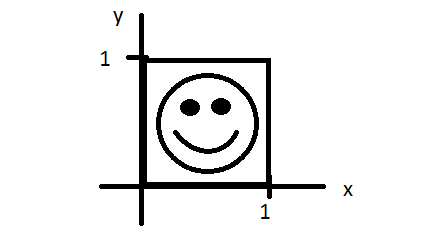
\includegraphics{smiley.png} \end{center}
\begin{enumerate}
\item $T: \mathbb{R}^2 \to \mathbb{R}^2$ reflects points across the vertical axis.
\item $T: \mathbb{R}^2 \to \mathbb{R}^2$ rotates points clockwise by $\pi/2$ (around the origin).
\item $T: \mathbb{R}^2 \to \mathbb{R}^2$ where $T(\vec{x})=A\vec{x}$ and $A=\begin{bmatrix}1 & 2 \\0&1 \end{bmatrix}$
\item $T: \mathbb{R}^2 \to \mathbb{R}^2$ where $T(\vec{x})=A\vec{x}$ and $A=\begin{bmatrix}3 & 0 \\0&2 \end{bmatrix}$
\item $T: \mathbb{R}^2 \to \mathbb{R}^2$ where $T(\vec{x})=A\vec{x}$ and $A=\begin{bmatrix}0 & -1 \\1&0 \end{bmatrix}$
\item $T: \mathbb{R}^2 \to \mathbb{R}^2$ where $T(\vec{x})=A\vec{x}$ and $A=\begin{bmatrix}0 & 0 \\0&1 \end{bmatrix}$
\end{enumerate}
\eq


\bq If a linear transformation, $T$, sends the vector $\colvec{2}{1}{1}$ to $\colvec{2}{-2}{2}$ and sends the vector $\colvec{2}{-1}{1}$ to $\colvec{2}{0}{2}$, find the following:
\begin{itemize}
\item $T\left(\colvec{2}{1}{0}\right)$ Hint: How can you write $\colvec{2}{1}{0}$ as a linear combination of  $\colvec{2}{1}{1}$ and $\colvec{2}{-1}{1}$.
\item $T\left(\colvec{2}{0}{1}\right)$
\item $T\left(\colvec{2}{a}{b}\right)$
\item Find the standard matrix presentation for $T$
\end{itemize}
\eq

\bq
Let $T_{\vec{0}}$ be the function from $V$ to $W$ such that $T(\vec{x})=\vec{0}_W$ for every $\vec{x} \in V$. Let $Id_V$ be the identity map on $V$, $Id_V(\vec{x}) = \vec{x}$ for every $\vec{x} \in V$.
\be
\item Prove that $T_{\vec{0}}$ is linear.
\item Prove that $Id_V$  is linear.
\ee
\eq

The \textbf{range} of a linear transformation $T:V \rightarrow W$ is the set of things in the codomain $W$ that are the output of $T$ for some input. That is $range(T)= \{\vec{y} \in W | \vec{y}=T(\vec{x}) \mbox{ for some } \vec{x} \in V\}$. The \textbf{null space}, or \textbf{kernel}, of a linear transformation $T:V \rightarrow W$ is the set of inputs that get mapped to the zero vector of $W$. That is $Null(T)=\{\vec{x}\in V | T(\vec{x}) = \vec{0_W}\}$.

\bq Is $\vec{b}=\colvec{3}{0}{2}{1}$ in the range of the linear transformation $T(\vec{x})=A\vec{x}$ where $A= \begin{bmatrix} 1&2 \\ 3 & 4\\0&0 \end{bmatrix}$? Justify your answer without doing any matrix operations. Hint: write the corresponding matrix equation as a vector equation.
\eq

\bq Let $A=\begin{bmatrix} 1&2&3 \\4&5&6 \end{bmatrix}$. Find the range and null space of $T$ where $T(\vec{x}) =A \vec{x}$. Remember to state the range and null space so that the reader can most easily verify whether a vector is in the set or not.
\eq

\bq Let $T$ from $\mathbb{R}^2$ to $\mathbb{P}_2$ be given by $T \left( \colvec{2}{a}{b} \right) = a +(a+b)t+(a-b)t^2$.
\begin{enumerate}
\item Prove $T$ is linear.
\item Compute the range of $T$.
\item Compute the null space of $T$.
\end{enumerate}
\eq

\bq Let $V$ be the vector space of polynomials in $x$ and $y$. \be \item Show the transformation $T$ that maps $f$ to $\dfrac{\partial f}{\partial x}$ is a linear transformation.
\item Compute the null space of $T$.
\item Compute the range of $T$.
\ee
\eq

\bq\label{rnss}
Let $T$ be a linear transformation from $V$ to $W$. Prove that $null(T)$ is a subspace of $V$.
\eq
\bq\label{rnss2}
Let $T$ be a linear transformation from $V$ to $W$. Prove that $range(T)$ is a subspace of $W$.
\eq
A function $f: C \rightarrow D$ is \textbf{one to one} if whenever $f(x)=f(y)$, then $x=y$. This means that each input gets sent to a different output by the function $f$. Alternately, you can say a one to one function does not map two different inputs to the same output.

A function $f:C \rightarrow D$ is \textbf{onto} if every element of $D$ has some input that is mapped to it. In other words, a map $f$ is onto if the range of $f$ is all of $D$.
\bq For each of the functions from $\mathbb{R}$ to $\mathbb{R}$ below state whether the function is either 1-1 but not onto, onto but not 1-1, 1-1 and onto, or not 1-1 and not onto.
\begin{enumerate}
\item $f(x) =e^x$
\item $f(x) =x$
\item $f(x) =x^2$
\item $f(x) =1-x$
\item $f(x) =x^2(1-x)$
\item $f(x) =sin(x)$
\item $f(x) =x^3$
\end{enumerate}
\eq

\bq Let $T$ from $\mathbb{R}^2$ to $\mathbb{P}_2$ be given by $T \left( \colvec{2}{a}{b} \right) = a +(a+b)t+(a-b)t^2$.
\begin{enumerate}
\item Is $T$ one-to-one?
\item Is $T$ onto?
\end{enumerate}
\eq

\bq Give an example of a linear transformation from $\mathbb{R}^2$ to $\mathbb{R}^3$ that is one to one.
\eq

\bq Give an example of a linear transformation from $\mathbb{R}^2$ to $\mathbb{R}^2$ that is onto.
\eq


\bq Give an example of a linear transformation from $\mathbb{R}^3$ to $\mathbb{R}^2$ that is onto.
\eq

\bq If the set of columns of a $m$ by $n$ matrix $A$ are linearly independent, does the set of columns of $A$ span all of $\mathbb{R}^m$?
\eq
\bq If the set of columns of a $m$ by $n$ matrix $A$ are linearly independent, is the range of $T(\vec{x})=A\vec{x}$ all of $\mathbb{R}^m$?
\eq

\begin{theorem} A linear transformation $T:V \rightarrow W$ is onto iff $range(T)=W$. \end{theorem}

\bq Prove that for $T$ a linear transformation from $V$ to $W$, \break $null(T)=\{ \vec{0} \}$ iff $T$ is 1-1.
\eq

\section{Applications}
\begin{annotation}
\endnote{This application section is meant to show how solution sets to linear systems of differential equations are a vector space (a subspace of the proper function space). Specifically, the differential equation can be thought of as a linear transformation and thus the homogeneous differential equations can be found as the null space of the linear transformation. The parallel between solution sets of homogeneous/non-homogenous systems of differential and linear equations is also highlighted.}
\end{annotation}

\begin{definition}
Let $\mathcal{C}^n(\mathbb{R},\mathbb{R})$, or simply $\mathcal{C}^n$ be the set of functions from $\mathbb{R}$ to $\mathbb{R}$ that are $n$ times continuously differentiable.
\end{definition}
\bq Let $a_1,a_2,a_3,a_4 \in \mathbb{R}$. A solution to the system of differential equations: $$\dfrac{dx}{dt} = a_1 \enskip x(t)+a_2 \enskip y(t)$$ $$\dfrac{dy}{dt} = a_3 \enskip x(t) +a_4 \enskip y(t) $$ is a choice of $x$ and $y$ as functions of $t$ such that both differential equations are satisfied.
\be
\item If the pair of functions $(g(t),h(t))$ is a solution to the system above, what does this imply about the derivatives of $g$ and $h$? Be very specific.

The solution set to the given set of differential equations will be a subset of the ordered pairs of differentiable functions; specifically the solutions will be in the set $(\mathcal{C}^2)^2=\{ (x(t),y(t))|x,y \in \mathcal{C}^2\}$.

\item Prove that the set of solutions to the system above is a subspace of the vector space $(\mathcal{C}^2)^2$.
\item If we consider the system of differential equations given by $$\dfrac{dx}{dt} = a_1 \enskip x(t)+a_2 \enskip y(t)$$ $$\dfrac{dy}{dt} = a_3 \enskip x(t) + 1  $$, is the set of solutions to this system a subspace of $(\mathcal{C}^2)^2$? Be sure to justify why or why not.
\item \item If we consider the system of differential equations given by $$\dfrac{dx}{dt} =  (x(t))^2 +a_2 \enskip y(t)$$ $$\dfrac{dy}{dt} = a_3 \enskip x(t) + +a_4 \enskip y(t)  $$, is the set of solutions to this system a subspace of $(\mathcal{C}^2)^2$? Be sure to justify why or why not.
\ee
\eq
The previous result is especially important in a differential equations class because finding the solution set of the system of differential equations reduces to finding a few solutions that spans a large enough space.

\bq \begin{enumerate}
\item Let $S$ be the set of solutions to the differential equation $a\dfrac{d^2x}{dt^2}+b\dfrac{dx}{dt}+c x(t)= 0$. Prove that $S=\{f \in F(\mathbb{R},\mathbb{R}) | a\dfrac{d^2f}{dt^2}+b\dfrac{df}{dt}+c f(t)= 0 \}$  is a subspace of $F(\mathbb{R},\mathbb{R})$.
\item If $f_1(t)$ and $f_2(t)$ are solutions to the differential equation $a\dfrac{d^2x}{dt^2}+b\dfrac{dx}{dt}+c (x(t))= g(t)$, then prove that $f_1-f_2$ is a solution to the homogeneous differential equation $a\dfrac{d^2x}{dt^2}+b\dfrac{dx}{dt}+c (x(t))= 0$.
\item Conclude that the solution set of the non-homogeneous differential equation is of the form $y(t)+s(t)$, where $y$ is a solution to the nonhomogeneous differential equation and $s(t) \in S$, where $S$ is the solution set to the homogeneous differential equation.
\end{enumerate}
\eq
The previous problem is analogous to your work on Question \ref{q7}.
\bq \be
\item Show that the transformation $T$ from $\mathcal{C}^2$ to $\mathcal{C}^2$ given by $T(f)=a\dfrac{d^2f}{dt^2}+b\dfrac{df}{dt}+c f(t)$ is linear.
\item What is $Null(T)$?
\ee
\eq

\chapter{Connecting Ideas}

\section{Basis and Dimension}
In the previous chapter, we saw that if a set $S$ spans a vector space $V$, then $S$ is big enough to write everything in $V$ (as a linear combination of $S$). We also saw that a linearly independent set $S$ had a unique way to represent elements in $span(S)$ (Question \ref{u}). A convenient and minimal way to describe a vector space is to give a set of vectors that spans all of $V$ but does not include anything extra.
\begin{definition} A basis for a vector space $V$ is a set of vectors that is linearly independent and spans $V$.
\end{definition}
In this way, a basis is big enough (spans $V$) and contains nothing extra (linearly independent).

\bq Can a set of 4 vectors be a basis for $\mathbb{R}^3$? Why or why not? Be sure to justify using ideas from Chapter 1 and not any theorems past this point.
\eq

\bq Can a set of 2 vectors be a basis for $\mathbb{R}^3$? Why or why not?
\eq

\begin{theorem}
If there exists a basis for a vector space $V$ with $n$ vectors, then every basis of $V$ must have exactly $n$ vectors.
\end{theorem}
The previous theorem does not imply that there is only one basis for a vector space, just that any two bases for the same vector space will have the exact same number of vectors. The idea that every basis for a vector space $V$ has the same number of vectors gives rise to the idea of dimension.
\begin{definition} If a vector space $V$ has a basis with a finite number of elements, $n$, then we say that $V$ has \textbf{dimension} $n$ or that $V$ is \textbf{$n$-dimensional}, also written as $dim(V)=n$. \end{definition}

\bq Show that $\{ \vec{e_1}, ... ,\vec{e_n} \}$ is a basis for $\mathbb{R}^n$ and thus that $\mathbb{R}^n$ is an $n$-dimensional vector space.
\eq

\bq Give a set of 3 different vectors in $\mathbb{R}^3$ that are not a basis for $\mathbb{R}^3$. Be sure to show why the set does not satisfy the definition of a basis.
\eq

\bq Give a basis for $\mathbb{P}_3$ and compute the dimension of $\mathbb{P}_3$.
\eq

\bq What is $dim(\mathbb{P}_n)$? Be sure to justify.
\eq

\bq Recall that the set $\{\vec{0} \}$ is the trivial vector space. What is a basis for $\{\vec{0} \}$? What is $dim(\{\vec{0} \})$?
\eq

\begin{theorem}
If $V$ is an $n$-dimensional vector space and $S$ is a set with exactly $n$ vectors, then $S$ is linearly independent if and only if $S$ spans $V$.
\end{theorem}

This is an \emph{enormously} helpful theorem since we know that a linearly independent set of $n$ vectors from a $n$-dimensional vector space is a basis (no need to show spanning). This goes the other way as well, namely if a set of $n$ vectors, $S$, spans a $n$-dimensional vector space, $V$, then $S$ is a basis for $V$ (no need to show linear independence).

\bq Prove that $\{ 1+t,t+t^2,1+t^2 \}$ is a basis for $\mathbb{P}_2$.
\eq

\bq Give two different bases for $M_{2 \times 2}$.
\eq

\bq What is the dimension of $Sym_{3 \times 3}$, the vector space of symmetric 3 by 3 matrices?
\eq

\bq What is the dimension of $Sym_{n \times n}$?
\eq

\bq What is the dimension of $\mathbb{P}$? Justify your answer.
\eq

\bq \be
\item Prove that $H=\{ \colvec{3}{t}{t}{0} | t \in \mathbb{R} \} $ is a subspace of $\mathbb{R}^3$.
\item Is $Span(\{ \colvec{3}{1}{0}{0} , \colvec{3}{0}{1}{0} \}) =H$?
\item What dimension is $H$?
\ee \eq

\subsection{rank and nullity}
Recall from Question \ref{rnss}, if $T: V \rightarrow W$ is linear, then $Null(T)$ and \break $range(T)$ are subspaces of $V$ and $W$ respectively.
\begin{definition}  The \textbf{rank} of a transformation $T$ is $dim(range(T))$ and the \textbf{nullity} of $T$ is $dim(Null(T))$. \end{definition}


\bq Let $A=\begin{bmatrix} 1&2&3 \\4&5&6 \end{bmatrix}$.
\be
\item Find $rank(T)$ and $nullity(T)$ where $T(\vec{x}) =A \vec{x}$.
\item Find a basis for $Null(T)$.
\item Find a basis for $range(T)$.
\ee
\eq

\bq Let $T$ from $\mathbb{R}^2$ to $\mathbb{P}_2$ be given by $T \left( \colvec{2}{a}{b} \right) = a +(a+b)t+(a-b)t^2$.
\begin{enumerate}
\item $rank(T)=$
\item $nullity(T)=$
\item Find a basis for $Null(T)$.
\item Find a basis for $range(T)$.
\end{enumerate}
\eq

\bq Let $T:\mathbb{P}_3 \rightarrow \mathbb{R}^2$ be given by $T(f)=\colvec{2}{f(0)}{f(1)}$. Compute $rank(T)$ and $nullity(T)$.
\eq

\begin{theorem}[Dimension Theorem] Let $T$ be a linear transformation from $V$ to $W$ with $V$ a $n$-dimensional vector space. $rank(T) + nullity(T)=n$.
\end{theorem}

If $T$ is a matrix transformation ($T(\vec{x})=A\vec{x}$), then the $rank(T)=\break rank(A)=dim(Col(A))$ and $nullity(T)=nullity(A)=dim(Null(A))$.

\bq Using Question \ref{q10} and other previous work, prove the Dimension Theorem for $T: \mathbb{R}^n \rightarrow \mathbb{R}^m$ given by $T(\vec{x})=A\vec{x}$, where $A$ is a $m$ by $n$ matrix.
\eq

\bq List out all possible echelon forms of 3 by 3 matrices using the symbols $\blacksquare$ for pivot, $*$ for non-pivot entry (possibly $0$) , and $0$ if an entry \underline{must} be $0$. For each form, give the rank of the matrix and the dimension of the null space.
\eq

\subsection{Coordinate Vectors relative to a basis}
Given an ordered basis $\beta =\{ \vec{v_1}, ...,\vec{v_k} \}$ of a vector space $V$, the \textbf{coordinate vector of $\vec{x}$ relative to $\beta$}, denoted $[\vec{x}]_\beta$, is a vector of the coefficients of the unique way to write $\vec{x}$ as a linear combination of $\beta$. Namely, if \break $\vec{x} = c_1 \vec{v_1}+c_2 \vec{v_2} +...+c_k \vec{v_k}$, then $[\vec{x}]_\beta = \colvec{4}{c_1}{c_2}{\vdots}{c_k}$.

\bq For each of the following vectors, compute $[\vec{v}]_{\beta}$ where $\beta =\{ \colvec{3}{0}{0}{1}, \colvec{3}{0}{1}{1},\colvec{3}{1}{1}{1} \}$
\begin{enumerate}
\item $\vec{v}=\colvec{3}{2}{2}{2}$
\item $\vec{v}=\colvec{3}{3}{0}{0}$
\item $\vec{v}=\colvec{3}{-1}{-1}{0}$
\item $\vec{v}=\colvec{3}{-2}{0}{3}$
\item $\vec{v}=\colvec{3}{a}{b}{c}$
\end{enumerate}
\eq

\bq
In the previous problem, you wrote out the coordinate vectors relative to $\beta =\{ \colvec{3}{0}{0}{1}, \colvec{3}{0}{1}{1},\colvec{3}{1}{1}{1} \}$. Note that the first three vectors you used form a basis as well, which we will call $\gamma =\{ \colvec{3}{2}{2}{2}, \colvec{3}{3}{0}{0},\colvec{3}{-1}{-1}{0} \}$.
\be
\item Compute  $[\vec{v}]_{\gamma}$ for $v=\colvec{3}{-2}{0}{3}$.
\item The coordinate vectors of $\gamma$ relative to $\beta$ can be used to make the \textbf{change of basis matrix} from $\beta$ to $\gamma$. Specifically, the change of basis matrix from $\beta$ to $\gamma$ is given by $[ [\vec{\gamma_1}]_\beta [\vec{\gamma_2}]_\beta [\vec{\gamma_3}]_\beta ] $.  Use your work from the previous question, to construct the change of basis matrix from $\beta$ to $\gamma$.
\item Multiplying by this change of basis matrix will convert a coordinate vector relative to $\beta$ to a coordinate vector relative to $\gamma$. Verify that if you multiply your change of basis matrix from $\beta$ to $\gamma$ by $[\vec{v}]_{\beta}$ you get $[\vec{v}]_{\gamma}$ where  $v=\colvec{3}{-2}{0}{3}$.
\ee
\eq
The above process of constructing a change of basis matrix works for any two bases of the same vector space (even if the vector space is not $\mathbb{R}^n$.

\bq For each of the following vectors, compute $[\vec{v}]_{\beta}$ where $\beta =\{ 1+t,t+t^2,1+t^2 \}$
\begin{enumerate}
\item $\vec{v}=2+2t$
\item $\vec{v}=4-t^2+t$
\item $\vec{v}=3$
\item $\vec{v}=t$
\item $\vec{v}=6t^2$
\end{enumerate}
\eq

The coordinate vector allows us to state problems in a vector space like $\mathbb{P}_n$ in the same way we state problems in $\mathbb{R}^n$.

\bq For each of the following vectors, compute $[\vec{v}]_{\beta}$ where $\beta =\{ \begin{bmatrix} 1&2\\3&4  \end{bmatrix}, \begin{bmatrix} 1&0\\0&1  \end{bmatrix}, \begin{bmatrix} 0&1\\1&0  \end{bmatrix}, \begin{bmatrix} 1&0\\0&0 \end{bmatrix} \}$
\begin{enumerate}
\item $\vec{v}=\begin{bmatrix} 1&1\\1&1  \end{bmatrix}$
\item $\vec{v}=\begin{bmatrix} 1&0\\1&1  \end{bmatrix}$
\end{enumerate}
\eq


\section{Invertible Matrices}

In this section, we will only consider square matrices. A matrix $A \in M_{n \times n}$ is \textbf{invertible} if there exists a matrix $B$ such that $AB=Id_n$ and $BA=Id_n$. The inverse matrix of $A$ is denoted $A^{-1}$. Be careful that you do not use the notation $A^{-1}$ until you have shown that $A$ is invertible.

\subsection{Elementary Matrices}

Recall that an elementary row operation on a matrix is an operation of the form:

\begin{itemize}
\item multiplying a row by a non-zero scalar
\item switching two rows
\item adding a multiple of one row to another row
\end{itemize}
Elementary matrices are obtained by performing an elementary operation on the identity matrix.
\bq Give the elementary matrix obtained by performing the given operation on $Id_3$:
\begin{itemize}
\item Scaling the first row by $\alpha$
\item Switching the second and third rows
\item Adding 3 times the 2nd row to the 1st row.
\item Adding 3 times the 1st row to the 2nd row.
\end{itemize}
\eq

\bq Check that your answer to the previous question does the desired operation by multiplying each of the four previous elementary matrices by $\begin{bmatrix} a&b&c\\d&e&f\\g&h&i \end{bmatrix}$. Which side do you multiply the elementary matrix on to correspond to row operations?
\eq

\bq Compute (and verify) the inverse of each of the elementary matrices from the previous problems. (Hint: Think about how you would go backwards for each of the elementary operations.
\eq

Your work on the previous questions should convince you that elementary matrices are invertible and that multiplying by an elementary matrix produces the same result as having performed the corresponding elementary row operation. Elementary matrices offer a way of keeping track of elementary operations.
\begin{theorem}
Elementary matrices are invertible and the inverse matrix is an elementary matrix corresponding to the inverse elementary operation.
\end{theorem}

\begin{theorem}
If $A$ and $B$ are invertible $n$ by $n$ matrices, then $AB$ is an invertible $n$ by $n$ matrix. Further, $(AB)^{-1} =B^{-1}A^{-1}$.
\end{theorem}

\bq\label{q11} Prove that if $A$ can be reduced to $Id_n$ by elementary row operations, then $A$ is invertible.
\eq

\bq Give all values of $k$ where $A=\begin{bmatrix} 1&0&2\\-1&k&4\\3&5&1 \end{bmatrix}$ will be invertible.
\eq

\bq Give all values of $k$ where $A=\begin{bmatrix} 1&0&2\\-1&k&4\\3&-1&1 \end{bmatrix}$ will be invertible.
\eq

\bq How many pivots must a matrix $A$ have in order to be row reducible to $Id_n$? Justify using previous results.
\eq

\bq Prove that if $A$ is invertible, then $A\vec{x} =\vec{b}$ has a unique solution for every $\vec{b} \in \mathbb{R}^n$.
\eq

\bq Prove or disprove: If $A$ and $B$ are invertible $n$ by $n$ matrices, then $A+B$ is invertible.
\eq

\bq Prove that if $A$ is invertible, then $A^T$ is invertible.
\eq

\subsection{Computing Inverses}
In general computing the inverse of a matrix takes more time and operations than solving a system of equations. For this reason, it is generally easier to find and solve a related system of equations problem than to compute the inverse matrix. We will outline a few ways to find inverse matrices and compute a few small examples.

\bq If a matrix $A$ is row reduced to $Id_n$ by elementary row operations corresponding (in order of use) to elementary matrices $E_1$, $E_2$, ... , $E_k$, give an expression for $A^{-1}$.
\eq

\bq Use your answer to the previous question to prove the following:

Any sequence of elementary row operations that reduces $A$ to $Id_n$ also transforms $Id_n$ into $A^{-1}$.
\eq

The previous result shows that computing inverses is equivalent to a row reduction problem. In particular, if $A$ is invertible, then reducing $[ A \enskip | \enskip Id_n]$ to reduced row echelon form will produce the matrix $[ Id_n \enskip | \enskip A^{-1}]$.

\bq\label{22inv} Use the idea above to compute the inverse of $\begin{bmatrix} a&b\\c&d \end{bmatrix}$. Be sure to note any assumptions you will need to make in order to reduce $[ A \enskip | \enskip Id_n]$ to $[ Id_n \enskip | \enskip A^{-1}]$.
\eq

\bq If $A=\begin{bmatrix}1& 0& 1 \\0&2&-1 \\ 0&6&-1\end{bmatrix}$, find $A^{-1}$ and check that $A A^{-1}=Id_3$.
\eq

\bq
If $A=\begin{bmatrix} 0&-1\\3&4 \end{bmatrix}$, find $A^{-1}$ and use your answer to solve $A\vec{x} = \vec{b}$ if:
\begin{enumerate}
\item $\vec{b} =\colvec{2}{3}{1}$
\item $\vec{b} =\colvec{2}{-1}{-2}$
\item $\vec{b} =\colvec{2}{0}{5}$
\item $\vec{b} =\colvec{2}{\alpha}{\beta}$
\end{enumerate}
\eq
\subsection{Invertible Matrix Theorem}
\bq In many texts there is a long list of equivalent conditions for when a square matrix is invertible. Below is a list of some of these conditions that we have talked about or proven. Go back through your notes and questions and cite when we connected two of the ideas in the list. For instance, parts $a)$ and $b)$ are linked by Question \ref{q11}
\eq

\begin{theorem}[The Invertible Matrix Theorem]\label{imt}
Let $A$ be a $n$ by $n$ matrix. The following are equivalent statements (either all True or all False):
\begin{enumerate}
\item $A$ is an invertible matrix.
\item $A$ is row equivalent to $Id_n$.
\item $A$ has $n$ pivots.
\item $rank(A)=n$
\item $nullity(A)=0$
\item $A\vec{x} =\vec{0}$ has only the trivial solution.
\item The linear transformation $\vec{x} \rightarrow A\vec{x}$ is one-to-one.
\item The linear transformation $\vec{x} \rightarrow A\vec{x}$ is onto.
\item $A\vec{x}=\vec{b}$ has a solution for every $\vec{b} \in \mathbb{R}^n$.
\item The columns of $A$ form a linearly independent set.
\item The columns of $A$ span $\mathbb{R}^n$.
\item The columns of $A$ are a basis for $\mathbb{R}^n$.
\item $A^T$ is invertible.
\end{enumerate}
\end{theorem}

\bq
Two important ideas in this course that have been tied to many different methods or ideas are 1) consistent systems of linear equations and 2) invertible matrices. These two ideas are a bit different though. Give an example of a consistent system of linear equations (in matrix equation form $A\vec{x} = \vec{b}$) where the coefficient matrix $A$ is a non-invertible square matrix.
\eq

\section{Invertible Linear Transformations}
\begin{annotation}
\endnote{This section and the next one on LU decomposition are examples of ideas that students who have successfully completed this course can pick up and use on thier own. They appear here because they can be quite useful.}
\end{annotation}

\begin{definition}
A linear transformation $T$ from $V$ to $W$ is invertible if there exists a linear transformation $U$ from $W$ to $V$ such that $T\circ U=Id_W$ and $U \circ T=Id_V$.
\end{definition}
Alternative definition:  A linear transformation $T$ from $V$ to $W$ is invertible if $T$ is one-to-one and onto.


\bq Let $A=\begin{bmatrix} 1&2&3 \\4&5&6 \end{bmatrix}$. Is $T:\mathbb{R}^3 \to \mathbb{R}^2$ given by $T(\vec{x})=A\vec{x}$ an invertible linear transformation?
\eq

\bq Let $T$ from $\mathbb{R}^2$ to $\mathbb{P}_2$ be given by $T \left( \colvec{2}{a}{b} \right) = a +(a+b)t+(a-b)t^2$. Is $T$ an invertible linear transformation?
\eq

\bq Let $T$ from $\mathbb{R}^3$ to $\mathbb{P}_2$ be given by $T \left( \colvec{3}{a}{b}{c} \right) = (a+c) +(a+b)t+(a-b)t^2$. Is $T$ an invertible linear transformation?
\eq

\section{LU factorization of matrices}
\begin{annotation}
\endnote{This section can be very important to applied mathematics since it relates to efficient computation, but some instructors choose to skip this for time reasons.}
\end{annotation}

\bq \begin{enumerate}
\item Reduce $A=\begin{bmatrix} 1&2 \\ 3&4\end{bmatrix}$ to \underline{echelon} form (not reduced row echelon form). How many row operations did you use?
\item Compute the elementary matrix (or matrices) corresponding to the row operation(s) from the previous part.
\item Compute the inverse of the elementary matrix from the previous problem and multiply the result by the echelon form you found in part $b)$. What is your result and why does this make sense?
\item Let $L$ be the inverse elementary matrix from part $c)$ and let $U$ be the echelon form from part $a)$. Solve $L\vec{y}=\vec{b}$ for $\vec{b}=\colvec{2}{1}{-1}$.
\item Now solve $U\vec{x}=\vec{y}$.
\item Now solve $A\vec{x}=\vec{b}$.
\end{enumerate}
\eq

\bq \begin{enumerate}
\item Reduce $A=\begin{bmatrix} 1&2&3\\ 4&5&6 \\ 7&8&9 \end{bmatrix}$ to \underline{echelon} form. How many row operations did you use?
\item Compute the elementary matrix (or matrices) corresponding to the row operation(s) from the previous problem.
\item Compute the inverse of the elementary matrix (or product of matrices) from part $b)$ and multiply your answer by the echelon form you found in part $a)$. What is your result and why does this make sense?
\item Let $L$ be the inverse elementary matrix product from part $c)$ and let $U$ be the echelon form from part $a)$. Solve $L\vec{y}=\vec{b}$ for $\vec{b}=\colvec{3}{1}{-1}{0}$.
\item Now solve $U\vec{x}=\vec{y}$.
\item Now solve $A\vec{x}=\vec{b}$.
\end{enumerate}
\eq

The preceding two problems can be generalized to show how row operations will conveniently reduce any matrix into a product of an upper- and a lower-diagonal matrix. This $LU$ decomposition has certain advantages when solving linear systems using a computer, especially for large systems.

\section{Determinants}
Determinants will be an incredibly useful tool in quickly determining several important properties of square matrices. We will first look at how to compute determinants and later outline the important properties that determinants have. While some of you may have been taught some rules for how to compute determinants of 2 by 2 and 3 by 3 matrices, I encourage you to understand how to compute determinants in general.
\subsection{Computing Determinants}
\begin{definition}
The \textbf{determinant} is a function from $n$ by $n$ matrices to the real numbers ($det:M_{n \times n} \rightarrow \mathbb{R}$). If $A$ is a 1 by 1 matrix, $A=[A_{1,1}]$, then $det(A)=A_{1,1}$. For $n \geq 2$, the determinant of a $n$ by $n$ matrix is given by the following formula in terms of determinants of $(n-1)$ by $(n-1)$ matrices:
$$det(A)=\sum_{j=1}^n (-1)^{1+j} (A)_{1,j} \enskip det(A^*_{1,j})$$
where $A^*_{i,j}$ is the $(n-1)$ by $(n-1)$ matrix obtained by deleting the $i$-th row and $j$-th column of $A$.

The term $(A)_{i,j}\enskip det(A^*_{i,j})$ is called the \textbf{$(i,j)$ cofactor of $A$}.

The range of the determinant is $\mathbb{C}$ if the entries of the matrix are complex.
\end{definition}
The above definition uses cofactor expansion along the first row.
\bq In this question, we will unpack the determinant formula above for a 2 by 2 matrix $A=\begin{bmatrix} a&b \\c&d \end{bmatrix}$.
\begin{enumerate}
\item Rather than using the summation notation of the formula above, write out the two terms in $det(A)$.
\item $A^*_{1,1}=$
\item $A^*_{1,2}=$
\item $(A)_{1,1}=$
\item $(A)_{1,2}=$
\item $(-1)^{1+1}=$
\item $(-1)^{1+2}=$
\item $det(A)=$
\end{enumerate}
\eq
Your answer to the previous problem will be useful in calculating determinants of 3 by 3 matrices.
\begin{theorem}
The determinant can be computed by cofactor expansion along any row or column. Specifically the cofactor expansion along the $k$-th row is given by $$det(A)=\sum_{j=1}^n (-1)^{k+j} (A)_{k,j} \enskip det(A^*_{k,j})$$
and the cofactor expansion along the $k$-th column is given by
$$det(A)=\sum_{i=1}^n (-1)^{i+k} (A)_{i,k} \enskip det(A^*_{i,k})$$
\end{theorem}

\question Use cofactor expansion along the first column of \break $A=\begin{bmatrix} a&b&c\\d&e&f\\g&h&i \end{bmatrix}$ to compute $det(A)$.

\question Use cofactor expansion along the second row of \break $A=\begin{bmatrix} a&b&c\\d&e&f\\g&h&i \end{bmatrix}$ to compute $det(A)$. Did you get the same answer as the previous question?

\question Compute the determinant of $B=\begin{bmatrix}g&h&i \\d&e&f\\ a&b&c \end{bmatrix}$. How does your answer compare with the previous problem?

\question Compute the determinant of $C=\begin{bmatrix} a&b&c\\3d&3e&3f\\g&h&i \end{bmatrix}$.

\question Compute the determinant of $D=\begin{bmatrix} a+kd&b+ke&c+kf\\d&e&f\\g&h&i \end{bmatrix}$.

\bq Compute the determinant of the following matrices:
\begin{enumerate}
\item $\begin{bmatrix} 3&0&1&0\\0&2&-1&4 \\-3&5&0&2\\2&2&2&-1 \end{bmatrix}$
\item $2\begin{bmatrix} 3&0&1&0\\0&2&-1&4 \\-3&5&0&2\\2&2&2&-1 \end{bmatrix}$
\end{enumerate}
\eq
\subsection{Properties of Determinants}

\bq Prove that $det(Id_n)=1$.
\eq

\bq Use your results from the previous subsection to state what the determinants of the different kinds of elementary matrices are. (You do not need to prove the general case, just give a clear, correct statement.)
\eq

\bq Prove that if $A$ has a row of zeros, then $det(A)=0$.
\eq

\begin{theorem}
\begin{enumerate}
\item If $A$ and $B$ are $n$ by $n$, then $det(AB)=det(A) det(B)$.
\item The determinant of an upper or lower triangular matrix is the product of its diagonal entries. $$det(L)=\prod_{i=1}^n L_{i,i}$$ $$det(U)=\prod_{i=1}^n U_{i,i}$$
\item The determinant of a diagonal matrix is the product of its diagonal entries. If $D$ is diagonal, then $$det(D)=\prod_{i=1}^n D_{i,i}$$
\item $det(A)=det(A^T)$
\item A matrix $A$ is invertible iff $det(A)\neq 0$. This property should be included in the Invertible Matrix Theorem. In fact, you should go write it in as part (n) of Theorem \ref{imt}.
\end{enumerate}
\end{theorem}

\begin{annotation}
\endnote{In the next problem, we use an elementary operation on columns. This is intentional. I take this as a time to remind students that everything we have been doing as far as row operations can be applied to deal with column operations. In this course we don't worry about considering both concepts all of the time in order to have time to deeply understand the relationships involving row operations. I also try to remind them that everything we have done so far more or less stems from row operations or can be taken from an abstract setting and applied as solving a system of linear equation (with row operations!!!).}
\end{annotation}
\bq Let $A=E_1 E_2 E_3$ be a four by four matrix, where
\begin{itemize}
\item $E_1$ is the elementary matrix that adds two times the 2nd column to the 3rd column
\item $E_2$ is the elementary matrix that switches the second and fourth rows
\item $E_3$ is the elementary matrix that scales the first row by $\frac{1}{2}$
\end{itemize}
Compute $det(A)$.
\eq

\bq Let $A\vec{x}=LU\vec{x}=\vec{b}$, where $L=\begin{bmatrix} 1&0&0\\-2&1&0\\2&-3&1 \end{bmatrix}$, \break $U=\begin{bmatrix} 3 &-1 &2\\0&1&-2\\0&0&5 \end{bmatrix}$, and $\vec{b}=\colvec{3}{1}{1}{1}$. Compute $det(L)$, $det(U)$, \break and $det(A)$. What relationship should these determinants have?
\eq

\bq Let $A=\begin{bmatrix} 1&2&3\\4&5&6\\0&1&-1 \end{bmatrix}$ and $\vec{b}=\colvec{3}{1}{1}{1}$.
\begin{enumerate}
\item Compute $det(A)$.
\item Let $A_1$ be the matrix obtained by replacing the first column of $A$ with $\vec{b}$. Compute $det(A_1)$.
\item By similar replacement of the second and third columns, find $A_2$ and $A_3$. Compute $det(A_2)$ and $det(A_3)$.
\item Solve $A\vec{x}=\vec{b}$.
\item Write $\colvec{3}{x_1}{x_2}{x_3}$ in terms of $det(A_1)$, $det(A_2)$, $det(A_3)$, and $det(A)$.
\end{enumerate}
\eq

The previous problem is an example of \textbf{Cramer's Rule}, which allows you to write the unique solution of $A\vec{x} =\vec{b}$ (for a square invertible matrix $A$) in terms of determinants.

\bq\label{ee} Prove: $det(A)=0$ iff $A\vec{x}=\vec{0}$ has solutions such that $\vec{x} \neq \vec{0}$.
\eq

\section{Eigenvalues and Eigenvectors}
\begin{annotation}
\endnote{Throughout this section, the students may ask about solving some of the algebraic equations using complex numbers. Only after Question \ref{q13} are complex numbers explicitly addressed. I typically take this as an opportunity to talk to students about the assumptions that may be implicit in problems and that if they think real versus complex would change the answer to the question, then they should consider and write up both cases (This always comes up by Question \ref{q14} at the latest). Many students do not have facility with solving algebraic problems with complex numbers and other students' presentations offer another time to expose them to these ideas. Your milage may vary.}
\end{annotation}
\begin{definition}
An \textbf{eigenvector} of a matrix $A$ is a nonzero vector $\vec{x}$ such that $A\vec{x}=\lambda \vec{x}$ for some scalar $\lambda$. The scalar $\lambda$ is called an \textbf{eigenvalue} of $A$ if there exists a nonzero solution to $A\vec{x}=\lambda \vec{x}$.
\end{definition}

\bq Which of the following vectors are an eigenvector of $A=\begin{bmatrix} 2&3\\3&2 \end{bmatrix}$? For any vectors that are eigenvectors of $A$, give the eigenvalue. \begin{enumerate}
\item $\vec{v_1}=\colvec{2}{1}{2}$
\item $\vec{v_2}=\colvec{2}{-1}{1}$
\item $\vec{v_3}=\colvec{2}{3}{-1}$
\item $\vec{v_4}=\colvec{2}{1}{1}$
\item $\vec{v_5}=\colvec{2}{0}{0}$
\end{enumerate}
\eq

\bq Let $A=\begin{bmatrix} 2&1\\-1&3 \end{bmatrix}$. Try to find an eigenvector with eigenvalue $3$. In other words, find a vector $\vec{v}$ such that $A\vec{v}=3\vec{v}$.
\eq

\bq Let $A=\begin{bmatrix} 3&4\\3&-1 \end{bmatrix}$. Try to find an eigenvector with eigenvalue $-3$. In other words, find a vector $\vec{v}$ such that $A\vec{v}=-3\vec{v}$.
\eq

\bq Prove: $det(A- \alpha Id)=0$ iff $\alpha$ is an eigenvalue. Hint: Look at Question \ref{ee}.
\eq

If $A$ is a $n$ by $n$ matrix, then $det(A- t Id)$ will be a $n$-th degree polynomial in $t$, which we call the \textbf{characteristic polynomial of $A$}. The previous question shows that finding roots of the characteristic polynomial is the same as finding eigenvalues.

\bq Find each of the following matrices: write out the characteristic polynomial, give all eigenvalues, and for each eigenvalue, find an eigenvector.
\begin{enumerate}
\item $\begin{bmatrix} 1&1 \\1&1 \end{bmatrix}$
\item $\begin{bmatrix} 1&-3 \\-3&1 \end{bmatrix}$
\item $\begin{bmatrix} 1&2 \\3&4 \end{bmatrix}$
\item $\begin{bmatrix} 1&2&3 \\4&5&6\\7&8&9 \end{bmatrix}$
\item $\begin{bmatrix} 4&-1&6\\2&1&6\\2&-1&8 \end{bmatrix}$
\item $\begin{bmatrix} 1&1&0&0\\1&1&0&0\\0&0&1&-3\\0&0&-3&1 \end{bmatrix}$
\end{enumerate}
\eq
\begin{annotation}
\endnote{Part e) of the previous problem is important for students to work through since it sets up Question \ref{q92}. Sometimes Question \ref{q92} can be done as an entire 50 minute class since it encapsulates a lot of understanding of dimension, eigenspaces, and previews diagonalizability.}
\end{annotation}

A root $\alpha$ of a polynomial (in $t$) has (algebraic) multiplicity $k$ if $k$ is the largest integer such that $(t-\alpha)^k$ is a factor.

\bq Prove that a nonzero vector, $\vec{v}$, is an eigenvector of $A$ with eigenvalue $\lambda$ if and only if $\vec{v}$ is in the null space of $A-\lambda Id$.
\eq

\bq Prove that if $\vec{v}$ is an eigenvector of $A$, then $\alpha \vec{v}$ is also an eigenvector of $A$ (when $\alpha \neq 0$).
\eq

\bq Prove that if $\vec{v_1}$ and $\vec{v_2}$ are eigenvectors of $A$ with the same eigenvalue, then $\vec{v_1}+\vec{v_2}$ is also an eigenvector of $A$. What is the eigenvalue of $\vec{v_1}+\vec{v_2}$?
\eq

\begin{definition}
If $\lambda$ is an eigenvalue of $A$, then the \textbf{eigenspace of $\lambda$}, $E_\lambda$, is the set of vectors $\vec{x}$ such that $(A-\lambda Id_n)\vec{x}=\vec{0}$. The previous two questions along with the inclusion of $\vec{0}$ give the following theorem.
\end{definition}
\begin{theorem} If $\lambda$ is an eigenvalue of $A \in M_{n \times n}$, then $E_\lambda$ is a subspace of $\mathbb{R}^n$.
\end{theorem}

\bq Prove that $dim(E_\lambda) \geq 1$ for every eigenvalue $\lambda$.
\eq

\question\label{q92} \begin{enumerate} \item Let $A =\begin{bmatrix} 2 &a&b\\0&2&c\\0&0&2 \end{bmatrix}$. Show that $A$ only has an eigenvalue of 2. What is the algebraic multiplicity of the eigenvalue 2?
\item Can you pick $a$, $b$, and $c$, so that the eigenspace of 2 has dimension 3? If so, give a choice of $a$, $b$, and $c$ that does so.
\item Can you pick $a$, $b$, and $c$, so that the eigenspace of 2 has dimension 2? If so, give a choice of $a$, $b$, and $c$ that does so.
\item Can you pick $a$, $b$, and $c$, so that the eigenspace of 2 has dimension 1? If so, give a choice of $a$, $b$, and $c$ that does so.
\end{enumerate}

\subsection{Diagonalizability}
\begin{definition}
A matrix $A$ is \textbf{diagonalizable} if there exists an invertible matrix $Q$ such that $A=QDQ^{-1}$ where $D$ is a diagonal matrix.
\end{definition}
\begin{theorem}
A matrix $A \in M_{n \times n}$ is diagonalizable iff $A$ has $n$ linearly independent eigenvectors. In fact, the matrix $Q$ that will diagonalize $A$ will have the $n$ linearly independent eigenvectors as its columns.
\end{theorem}
The question becomes when can we find $n$ linearly independent eigenvectors for a matrix $A$. It turns out that \textbf{\underline{if you can}} find $n$ linearly independent eigenvectors for $A$, then the matrix $Q$ has columns given by these eigenvectors and the diagonal matrix will have the eigenvalues on the diagonal. In particular, if the $i$-th column of $Q$ has eigenvalue $\lambda_i$, then $D_{i,i} = \lambda_i$.

\bq Can you diagonalize $A=\begin{bmatrix} -1&2\\-2&4 \end{bmatrix}$? If so, give a basis of eigenvectors, give corresponding choices for $Q$, $Q^{-1}$, and $D$, then use these to demonstrate how $A=QDQ^{-1}$. \eq

\bq\label{q14} Can you diagonalize $A=\begin{bmatrix} 1&-1\\1&1 \end{bmatrix}$? If so, give a basis of eigenvectors, give corresponding choices for $Q$, $Q^{-1}$, and $D$, then use these to demonstrate how $A=QDQ^{-1}$. \eq

\bq Prove that if $\vec{v_1}$ is an eigenvector with eigenvalue $\lambda_1$ and $\vec{v_2}$ is an eigenvector with eigenvalue $\lambda_2 \neq \lambda_1$, then $\{ \vec{v_1},\vec{v_2} \}$ is linearly independent.  \eq

The following theorem relies on the preceding question and the fact that the dimension of every eigenspace is at least 1.
\begin{theorem}
If a $n$ by $n$ matrix $A$ has $n$ distinct eigenvalues, then $A$ is diagonalizable.
\end{theorem}

\bq The converse of this theorem is not true in that there diagonalizable matrices that do not have distinct eigenvalues. Give an example of a matrix that is diagonalizable but does not have distinct eigenvalues. Remember that diagonal matrices are diagonalizable. \eq

\begin{theorem}
A $n$ by $n$ matrix $A$ is diagonalizable iff the sums of the dimensions of its eigenspaces is $n$.
\end{theorem}

\bq Give an example of a matrix that is not diagonalizable. Justify your claim.
\eq

\bq Let $A$ be a $4$ by $4$ matrix. \begin{enumerate} \item How many eigenvalues can $A$ have?
\item For each of the possible number of eigenvalues in the previous part, write out all of the possible dimensions of each of the eigenspaces. For instance: if $A$ has 4 distinct eigenvalues, then the only possibility is that each eigenspace has dimension 1 (why is that?).
\item Which of the cases from the previous problem correspond to $A$ being diagonalizable?
\end{enumerate}
\eq
\subsection{Eigenvalues and Eigenvectors of Linear Transformations}
The structure of eigenvalues, eigenvectors, and even diagonalizability can be generalized to linear transformations if we consider a square matrix $A$ as a transformation $\vec{x} \rightarrow A\vec{x}$.

\begin{definition}
An \textbf{eigenvector} of a linear transformation $T:V \rightarrow V$ is a nonzero vector $\vec{x} \in V$ such that $T(\vec{x})=\lambda \vec{x}$ for some scalar $\lambda$. The scalar $\lambda$ is called an \textbf{eigenvalue} of $T$ if there exists a nonzero solution to $T(\vec{x}) = \lambda \vec{x}$.
\end{definition}

\bq Examine each of the following transformations of $\mathbb{R}^2$ geometrically and find all eigenvalues and eigenvectors of the transformation. You should not try to construct and use a transformation matrix but rather think about what kinds of vectors will be mapped to a scalar multiple of themselves. Only non-zero vectors that are mapped to a scalar multiple of themselves are eigenvectors.
\begin{enumerate}
\item $T_1$ flips points over the horizontal axis.
\item $T_2$ flips points over the line $y=mx$.
\item $T_3$ rotates points by $\pi$ counterclockwise.
\item $T_4$ rotates points by $\frac{\pi}{3}$ counterclockwise.
\item $T_5$ shears points horizontally by $2$. In other words, $T_5(\vec{e_1})=\colvec{2}{1}{0}$ and $T_5(\vec{e_2})=\colvec{2}{2}{1}$.
\item $T_6$ projects points onto the vertical axis.
\end{enumerate}
\eq

\bq What are the eigenvalues and eigenvectors of the transformation $T: \mathbb{P} \rightarrow \mathbb{P}$ given by $T(f) =\dfrac{df}{dt}$?
\eq

\bq Let $T$ be the transformation of $\mathbb{R}^2$ given by $T(\vec{x})=A\vec{x}$ with $A=\begin{bmatrix}0&2\\-2&0 \end{bmatrix} $. Describe geometrically what the linear transformation $T$ does.
\eq

\bq\label{q13} What are the eigenvalues and eigenvectors of $A=\begin{bmatrix}0&2\\-2&0 \end{bmatrix} $? You need to consider complex numbers for both the eigenvalues and eigenvectors. Be sure to check your eigenvalues and eigenvectors.
\eq

\bq What do you think the scalar multiplication by $2i$ is doing in the previous problem?
\eq

\bq Let $T$ be the linear transformation from $\mathbb{R}^2$ to $\mathbb{R}^2$ that rotates around the origin by $\frac{\pi}{2}$ clockwise and then scales vectors by a factor of 2. Find $A$, the standard matrix for $T$ and determine if $A$ is diagonalizable.
\eq

\bq Let $T$ be the linear transformation from $\mathbb{R}^2$ to $\mathbb{R}^2$ that rotates around the origin by $\theta$ counterclockwise. Find $A$, the standard matrix for $T$ (in terms of $\theta$).

Determine for which values of $\theta$ $A$ is diagonalizable.
\eq

\chapter{Inner Product Spaces}
\begin{annotation}
\endnote{I do not always get to this chapter of material but I have used this as work for exceptional students and for students seeking honors projects.}
\end{annotation}
\section{Inner Products}
Recall  the dot product of $\vec{v} =\colvec{4}{v_1}{v_2}{\vdots}{v_n} \in \mathbb{R}^n$ and $\vec{w} =\colvec{4}{w_1}{w_2}{\vdots}{w_n} \in \mathbb{R}^n$ is just the sum of the products of the components. Namely,
$$\vec{v} \cdot \vec{w} =\sum_{i=1}^n v_i w_i  =\vec{v}^T \vec{w}$$
The dot product of a vector $\vec{x} \in \mathbb{R}^n$ with itself gives the length of the vector squared, $\vec{x} \cdot \vec{x} = ||\vec{x}||^2$. The dot product is the familiar example of an inner product on a real vector space.

Remember that if $z = a+b i \in \mathbb{C}$, the conjugate of z is denoted $\overline{z}$ and computed as $\overline{z} = a -b i $.
\begin{definition}
An \textbf{inner product} on a vector space $V$ is a function from $V \times V$ to $\mathbb{R}$ for real vector spaces ($\mathbb{C}$ for complex vector spaces), denoted by $\langle *,*\rangle$, such that for all $\vec{x},\vec{y},\vec{z} \in V$ and $c \in \mathbb{R}$ (or $\mathbb{C}$):
\begin{enumerate}
\item $\langle \vec{x},\vec{y} \rangle=\langle \vec{y},\vec{x} \rangle$ (or $\langle \vec{x},\vec{y} \rangle=\overline{\langle \vec{y},\vec{x} \rangle}$ for $\mathbb{C}$).
\item $c \langle \vec{x},\vec{y} \rangle=\langle c\vec{x},\vec{y} \rangle$ and $ \langle \vec{x}+\vec{z},\vec{y} \rangle=\langle \vec{x},\vec{y} \rangle+\langle \vec{z},\vec{y} \rangle$
\item $\langle \vec{x},\vec{x} \rangle \geq 0$.
\end{enumerate}
A vector space with a defined inner product is called an \textbf{inner product space}.
\end{definition}

\begin{example}
\begin{enumerate}
\item $\mathbb{R}^n$ with the dot product defined above is an inner product space.
\item $C([0,1])$, the set of continuous functions on the interval $[0,1]$ is an inner product space when $$\langle f,g \rangle = \int_0^1 f(t)g(t) \enskip dt$$
\item Frobeinus Inner Product on Matrices: If $A,B \in M_{m \times n}(\mathbb{R}), then $$\langle A,B \rangle = \sum_{i=1}^{m}\sum_{j=1}^{n} A_{i,j} B_{i,j}$ is an inner product on $M_{m \times n}(\mathbb{R})$.
\end{enumerate}
\end{example}


\begin{definition} Two vectors $\vec{x}$ and $\vec{y}$ in an inner product space are \textbf{orthogonal} if $\langle \vec{x} ,\vec{y} \rangle=0$. \end{definition}

\bq Find 3 different vectors that are orthogonal to $\colvec{2}{1}{2}$.
\eq

\bq Find 3 different vectors that are orthogonal to $\colvec{3}{1}{2}{-1}$.
\eq

\bq Find a vector in $C([0,1])$ that is orthogonal to $f(t)=t$.
\eq

\bq Find a vector in $C([0,1])$ that is orthogonal to $f(t)=1$.
\eq

\bq Find a vector in $ M_{2 \times 3}(\mathbb{R})$ that is orthogonal to $A=\begin{bmatrix}0&2&1\\1&-3&0 \end{bmatrix}$. \eq
\begin{definition}
For vectors in $\mathbb{R}^n$, the \textbf{projection} of $\vec{x}$ onto $\vec{y}$ computed with the following: $$proj_{\vec{y}} \vec{x} = \left( \frac{\vec{x} \cdot \vec{y}}{\vec{y} \cdot \vec{y}} \right) \vec{y}$$
\end{definition}
\bq
\be
\item Compute $proj_{\vec{u}}\vec{v}$ with $\vec{u} = \langle 2,2 \rangle$ and $\vec{v} = \langle 1,3 \rangle$.
\item Plot $\vec{u}$, $\vec{v}$, and $proj_{\vec{u}} \vec{v}$ starting at the origin.
\item Write a few sentences about what the projection measures geometrically.
\ee
\eq
Inner product spaces are useful because the same argument we made in the previous problem about how much of one vector is in the direction of another can be generalized to vector spaces that do not have the geometric ideas of arrows in space.

\section{Orthogonal Complements}
A set of vectors is \textbf{orthogonal} if every pair of distinct vectors in the set is orthogonal.

Let $W$ be a subspace of an inner product space $V$. The orthogonal complement of $W$, denoted $W^\bot$, is the set of vectors in $V$ that are orthogonal to every vector in $W$.
\bq Let $W=span(\{ \colvec{2}{1}{1} \})$. What is $W^\bot$?
\eq
\bq Let $W=span(\{ \colvec{3}{1}{0}{0},\colvec{3}{0}{1}{0} \})$. What is $W^\bot$?
\eq
\bq Let $W=span(\{ f(t) = t \})$ be a subspace of $C([0,1])$. What is $W^\bot$?
\eq
\bq Prove that if $W$ is a subspace of an inner product space $V$, then $W^\bot$ is a subspace of $V$.
\eq

\section{Orthonormal Bases.}
The elementary vectors of $\mathbb{R}^n$,  $\{ \vec{e_1},\vec{e_2}, ... ,\vec{e_n}\}$, form a basis for $\mathbb{R}^n$. Even better than that, the basis has only unit vectors and is orthogonal as a set (each pair of vectors is orthogonal to each other). These properties are very fundamental to how you worked with vectors before you started this class and why $\mathbb{R}^n$ has such nice geometric intuition built in. The fundamental idea of this section is understanding a procedure for how to \textbf{\emph{build}} a basis that is an orthogonal set and has vectors of \lq\lq length \rq\rq one.

\bq In this question, you will build an orthonormal basis of $\mathbb{R}^3$ from the ordered set $ \beta = \{ \colvec{3}{1}{2}{2}, \colvec{3}{3}{0}{0},\colvec{3}{-1}{-1}{0} \}$. Orthonormal means that the set is orthogonal and contains only unit vectors.
\be
\item We will construct the orthonormal basis $\gamma = \{ \vec{\gamma_1}, \vec{\gamma_2} , \vec{\gamma_3} \}$ by going through the elements in $\beta$ in order. In other words, we will consider $\vec{\beta_1} = \colvec{3}{1}{2}{2}$ first. Find $\gamma_1$, a unit vector in the direction of $\vec{\beta_1}$. This will be our first unit basis vector in $\gamma$.
\item We now want to consider $\vec{\beta_2}= \colvec{3}{3}{0}{0}$. Is $\vec{\beta_2}$ orthogonal to $\vec{\gamma_1}$?
\item We didn't get lucky so we will have to take out the part of $\vec{\beta_2}$ that is NOT orthogonal to $\vec{\gamma_1}$. In other words, we need to find the projection of $\vec{\beta_2}$ onto $\vec{\gamma_1}$. Compute $proj_{\vec{\gamma_1}} \vec{\beta_2}$.
\item In order to take out the part of $\vec{\beta_2}$ that is NOT orthogonal to $\vec{\gamma_1}$, we should subtract $proj_{\vec{\gamma_1}} \vec{\beta_2}$ from $\vec{\beta_2}$. Find $\vec{\beta_2} - proj_{\vec{\gamma_1}} \vec{\beta_2}$ and verify that this difference IS orthogonal to $\vec{\gamma_1}$.
\item Since $\vec{\beta_2} - proj_{\vec{\gamma_1}} \vec{\beta_2}$ is orthogonal to $\vec{\gamma_1}$, we define $\vec{\gamma_2}$ be the unit vector in the direction of $\vec{\beta_2} - proj_{\vec{\gamma_1}} \vec{\beta_2}$. Write out the set $\{ \vec{\gamma_1},\vec{\gamma_2} \}$.
\item All that's left to do is take $\vec{\beta_3}$ and make $\vec{\gamma_3}$, a unit vector that is orthogonal to both $\vec{\gamma_1}$ and $\vec{\gamma_2}$. Find the appropriate projections of $\vec{\beta_3}$ in order to subtract out the parts of $\vec{\beta_3}$ that is not orthogonal to $\vec{\gamma_1}$ and $\vec{\gamma_2}$. Then find the unit vector in the direction of the difference to get $\vec{\gamma_3}$.
\item Verify that $\gamma = \{ \vec{\gamma_1}, \vec{\gamma_2} , \vec{\gamma_3} \}$ is an orthonormal basis for $\mathbb{R}^3$.
\ee
\eq

\bq Go through the same process above to create an orthonormal basis of $\mathbb{P}_2$ from the basis $\beta = \{ 1,t,t^2\}$ using the inner product and projection formula given by $$\langle f,g \rangle = \int_0^1 f(t)g(t) \enskip dt$$ and $$proj_{\vec{y}} \vec{x} = \left( \frac{\langle \vec{x},\vec{y}\rangle}{\langle \vec{y},\vec{y}\rangle} \right) \vec{y}$$
\eq



\backmatter

\begin{annotation}
\chapter{Notes to the Instructor}
\renewcommand\notesname{}
\vspace{-2cm}
\begingroup
%\setlength{\parindent}{0pt}% Don't know what this does.  DMC
\setlength{\parskip}{2ex}
\renewcommand{\enotesize}{\normalsize}
\theendnotes
\endgroup
\end{annotation}


\end{document}
